% (c) 2012 -2014 Dimitrios Vrettos - d.vrettos@gmail.com
% (c) 2014 Claudio Carboncini - claudio.carboncini@gmail.com
% (c) 2014 Daniele Masini - d.masini.it@gmail.com

\chapter{Numeri naturali}

\section{L'origine dei numeri}

L'origine del sistema dei numeri naturali si perde nella notte dei tempi. Non abbiamo
documenti sufficienti per capire come l'uomo li abbia costruiti o scoperti; è possibile
che il nostro sistema di numerazione sia nato contemporaneamente al linguaggio stesso
della specie umana. Sono stati ritrovati tronchi fossili risalenti a più di trentamila
anni fa, recanti delle incisioni a distanza regolare. In particolare, è stato ritrovato un
osso di babbuino, detto ``Osso di Ishango'' (figura \ref{fig:ishango})
\footnote{\url{http://it.wikipedia.org/wiki/Osso_d'Ishango}} in quanto è stato rinvenuto presso la città di
Ishango nel Congo tra il Nilo e il lago Edoardo, che riporta delle tacche disposte
in modo tale da farci pensare che rappresentino dei numeri o dei calcoli. L'osso risale a
un periodo tra il~$20\,000$~\aC\ e il~$18\,000$~\aC

\begin{wrapfloat}{figure}{r}{0pt}
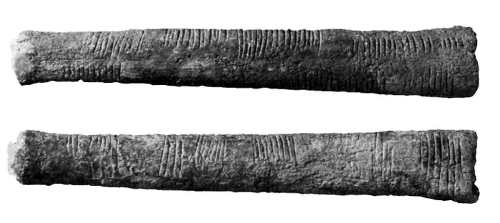
\includegraphics[scale=0.35]{/part01/chap01/fig001.png}
\caption{Osso di Ishango}
\label{fig:ishango}
\end{wrapfloat}
Possiamo immaginare che i pastori per contare i capi del proprio gregge, facessero delle
tacche su dei bastoni mano a mano che le pecore entravano nel recinto una alla volta: una
tacca per ogni pecora. Tuttavia, questo metodo di associazione uno ad uno (una tacca per
una pecora) non è efficace per greggi, o oggetti da contare, di grandi dimensioni. Si
immagini, per esempio, la difficoltà di tracciare cinquecento tacche su un bastone. È
possibile allora che per rappresentare numeri grandi si siano cominciati a usare simboli
specifici che richiamassero alla mente i numeri grandi e che contemporaneamente siano
state fissate alcune regole per associare questi simboli.

Sappiamo per certo che circa~6\,000 anni fa gli antichi Egizi scrivevano, incidendo sulla
pietra, i numeri utilizzando geroglifici per le potenze di~10:

% (c) 2012 Dimitrios Vrettos - d.vrettos@gmail.com
% Numeri egiziani
\begin{table}[!h]
  \begin{center}
    \begin{tabular}{ccccccc}
      \toprule
	\begin{hieroglyph}{\leavevmode \loneSign{\Aca GC/42/}}\end{hieroglyph} &  %
	\begin{hieroglyph}{\leavevmode \loneSign{\Aca GI/40/}}\end{hieroglyph} &%
	\begin{hieroglyph}{\leavevmode \loneSign{\Aca GD/84/}}\end{hieroglyph} &%
	\begin{hieroglyph}{\leavevmode \loneSign{\Aca GM/43/}}\end{hieroglyph} &%
	\begin{hieroglyph}{\leavevmode \loneSign{\Aca GV/32/}}\end{hieroglyph} &%
	\begin{hieroglyph}{\leavevmode \loneSign{\Aca GV/51/}}\end{hieroglyph}&%
	\begin{hieroglyph}{\leavevmode \loneSign{\Aca GZ/32/}}\end{hieroglyph}\\
      \midrule
	1\,000\,000   & 100\,000 & 10\,000 & 1\,000 & 100 & 10 & 1\\
      \bottomrule
    \end{tabular}
  \end{center}
\end{table}
\vspace{-4ex}
Ripetendo questi simboli è possibile scrivere, per esempio, il numero~$\np{3673}$ così:

\vspace{-2ex}% (c) 2012 Dimitrios Vrettos - d.vrettos@gmail.com
  \begin{center}
    \begin{hieroglyph}{\leavevmode \loneSign{\Aca GM/43/}\HinterSignsSpace
\loneSign{\Aca GM/43/}\HinterSignsSpace
\loneSign{\Aca GM/43/}\HinterSignsSpace
\Cadrat{\CadratLineI{\Aca GV/32/\hfill\Aca GV/32/\hfill\Aca GV/32/}\CadratLine{\Aca GV/32/\hfill\Aca GV/32/\hfill\Aca GV/32/}}\HinterSignsSpace
\Cadrat{\CadratLineI{{\Hsmaller\Hsmaller\Aca GV/51/}\hfill{\Hsmaller\Hsmaller\Aca GV/51/}\hfill{\Hsmaller\Hsmaller\Aca GV/51/}}\CadratLine{\Aca GV/51/\hfill\Aca GV/51/\hfill\Aca GV/51/\hfill\Aca GV/51/}}\HinterSignsSpace
\loneSign{\Aca GZ/32/}\HinterSignsSpace
\loneSign{\Aca GZ/32/}\HinterSignsSpace
\loneSign{\Aca GZ/32/}}\end{hieroglyph}
  \end{center}\vspace{-2ex}

I Romani usavano invece sette simboli con i quali, seguendo determinate regole,
rappresentavano qualunque numero. I simboli sono~$I=1$, $V=5$, $X=10$, $L=50$, $C=100$, $D=500$, $M=\np{1000}$.
La scrittura~$MM$ rappresenta il valore~$\np{1000}+\np{1000} = \np{2000}$, mentre~$VI$ rappresenta~$5+1=6$ ed invece~$IV$ rappresenta~$5-1=4$.

\section{Il sistema di numerazione decimale posizionale}
Il modo di scrivere i numeri dei Romani risultava piuttosto complicato sia nella scrittura
dei numeri sia nell'esecuzione dei calcoli. Il sistema tutt'oggi utilizzato per la scrittura dei numeri fa uso dei soli dieci simboli~0, 1, 2, 3, 4, 5, 6, 7, 8, 9, che vengono detti \emph{cifre}. Un numero è rappresentato da una sequenza ordinata di tali cifre (eventualmente anche ripetute).

Per rappresentare il numero dieci, che segue il~9, non si fa uso di un simbolo diverso ma si scrivono due cifre: il simbolo 1 e il simbolo 0 alla sua destra. Per chiarire questo metodo utilizziamo un pallottoliere (figura~\ref{fig:pallottoliere}) con aste verticali capaci di contenere fino a~9 dischetti: per rappresentare il numero~10 dispongo un dischetto nell'asta a sinistra e svuotando quella immediatamente alla sua destra: il numero dieci viene rappresentato dalla scrittura~10 che indica appunto 1 dischetto nella seconda asta (iniziando il conteggio da quella più a destra) e 0 in quella immediatamente a destra.

\begin{wrapfloat}{figure}{r}{0pt}
% (c) 2012 Dimitrios Vrettos - d.vrettos@gmail.com
% pallottoliere

\newcommand{\base}{%
  \filldraw[fill=black!90, draw=gray!80,rounded corners,shading=radial, inner color=white, outer color=gray!90]%
    (-2.4cm, -0.2cm) rectangle (2.4cm,0.4cm);
}

\newcommand{\aste}{%
  \fill[fill=black!90,rounded corners,shading=radial, inner color=white, outer color=gray!90]%
    (-1.25mm,3mm) rectangle (1.25mm,4.3cm);
}

\newcommand{\disco}{%
    \filldraw[fill=gray!20,draw=gray, rounded corners, shade,shading=radial, inner color=white, outer color=blue!50]%
      (-.6cm, .4cm) rectangle (.6cm,0.8cm);
}
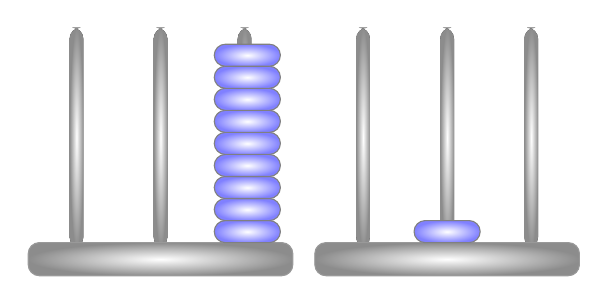
\begin{tikzpicture}[scale=.7]
  \foreach \n/\a in {-15.25mm,0,15.25mm,36.75mm,52mm,67.25mm}{
    \begin{scope}[xshift=\a]
      \aste
    \end{scope}
  }

  \foreach \n/\x in {1/0cm,2/5.2cm}{%
    \begin{scope}[xshift=\x]
	\base
    \end{scope}
  }
  
  \foreach \n/\y in {0,.4cm,...,3.2cm}{%
    \begin{scope}[xshift=15.75mm,yshift=\y]
	\disco
    \end{scope}
  }   	
	
  \foreach \n/\z in {0}{%
    \begin{scope}[xshift=52mm,yshift=\z]
      \disco
    \end{scope}
  }

\end{tikzpicture}

\caption{Il pallottoliere}
\label{fig:pallottoliere}
\end{wrapfloat}

I dischetti sull'ultima asta rappresentano il numero~9; un dischetto sulla penultima
rappresenta il numero~10. Per rappresentare il numero cento si fa uso della scrittura~100.
Ovvero si sposta il numero~1 ancora a sinistra ponendo uno 0 nel posto lasciato vuoto.

Questo metodo rappresenta i numeri dando ad ogni cifra un peso differente a seconda della posizione che essa occupa all'interno della rappresentazione del numero stesso: ogni posizione occupata da una cifra vale 10 volte di più rispetto a quella che si trova immediatamente alla sua destra.
La rappresentazione di un numero è quella che si ottiene riportando il numero di dischetti presenti in ogni asta dell'abaco, uno accanto all'altro. Per esempio, se ci sono soltanto 3 dischetti nella terza asta il numero in cifre è~$300$, mentre la scrittura~$219$ indica 2 dischetti nella terza asta, 1 nella seconda e 9 nella prima.
Il sistema di numerazione che utilizziamo, detto \emph{sistema decimale}, si basa sulle potenze di~10 (sezione~\ref{sect:potenza}), che è la base dei pesi assegnati alle posizioni occupate dalle cifre.

Nel pallottoliere ciascuna asta indica una potenza di dieci. Il valore di un numero si ottiene moltiplicando ciascuna cifra per il suo peso e sommando i valori ottenuti.

Per esempio, tre dischetti nella terza asta rappresentano il numero~$~3\cdot 10^2=300$.
Il numero~$219$ si rappresenta tenendo conto di questa scrittura~$~2\cdot 10^2+1\cdot 10+9$.

Per quanto detto, il sistema di numerazione che usiamo è decimale o a base dieci, perché
utilizza dieci simboli (cifre) per rappresentare i numeri, e posizionale perché una stessa cifra
assume un peso (valore) diverso a seconda della posizione che essa occupa.

\section{I numeri naturali}

I primi numeri che abbiamo usato sin da bambini per contare gli oggetti o le persone si
chiamano \emph{numeri naturali}
\[ 0\text{,~}1\text{,~}2\text{,~}3\text{,~}4\text{,~}5\text{,~}6\text{,~}7\text{,~}8\text{,~}9\text{,~}10\text{,~}11\text{,~}12\text{,~}13\text{,~}\dots \]
L'insieme di tutti questi numeri si indica con la lettera~$\insN$.

Cosa hanno in comune le dita di una mano, con~5 mele, 5~penne, 5~sedie? Evidentemente
il numero~5. Una caratteristica cioè che è comune a tutti gli insiemi formati da~5
oggetti. Questa caratteristica può essere vista come un oggetto a sé stante, un oggetto
astratto di tipo matematico.

Ma i numeri naturali non servono solo per indicare quanti oggetti ci sono (aspetto
\emph{cardinale} del numero), vengono usati anche per rappresentare l'ordine con cui si
presentano gli oggetti, (aspetto \emph{ordinale}), l'ordine per esempio con cui i corridori
arrivano al traguardo: primo, secondo, terzo, \ldots

Nonostante i numeri naturali e le operazioni su di essi ci vengano insegnati fin da
piccoli, e nonostante l'umanità li usi da tempi antichissimi una loro piena comprensione
non è semplice, come dimostra il fatto che ancora oggi i matematici ne discutono. Il
dibattito su cosa siano i numeri e su cosa si fondano è stato particolarmente animato nei
primi decenni del $XX$~secolo, quando ne hanno discusso matematici e filosofi come Frege,
Peano, Russell, Hilbert e tanti altri. Oggi ci sono diversi punti di vista.

\subsection{Rappresentazione geometrica}
I numeri naturali possono essere rappresentati su una semiretta: si identifica il numero~0
con l'origine della semiretta, come verso di percorrenza si prende quello da sinistra
verso destra e come unità di misura un segmento~$\overline{AB}$. Si riporta questa unità di misura
più volte partendo dall'origine e a ogni passo si va al numero successivo.
\begin{center}
 % (c) 2012 Dimitrios Vrettos - d.vrettos@gmail.com

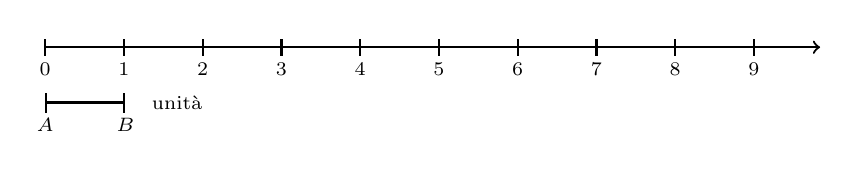
\begin{tikzpicture}
\begin{scope}[thick,font=\scriptsize]
	\draw[->] (0,0)  - -  (280pt,0) node[above]{$\insN$};
% 	\draw(1,-3pt) -- (1,3pt) node[below]{$1$};	
		\foreach \n in {0,1,2,...,9}{%
        	\draw (\n,-3pt) -- (\n,3pt)   node [below=5pt] {$\n$};}

		\draw[|-|]node [below=22pt]{$A$}(0,-20pt)--(29pt,-20pt) node[below=2pt]{$B$};

\end{scope}
\node [right,font=\scriptsize] at (+35pt,-20pt) {unit\`a};
\end{tikzpicture}

\end{center}

Ogni numero naturale si costruisce a partire dal numero~0 e passando di volta in volta al
numero successivo: 1 è il successore di~0, 2~è il successore di~1, 3~è il successore di~2,
ecc. Ogni numero naturale ha il successore e ogni numero, a eccezione di~0, ha il
precedente. L'insieme~$\insN$ ha~0 come elemento minimo e non ha un elemento massimo.

I numeri rappresentati sulla retta sono sempre più grandi man mano che si procede da
sinistra verso destra. Ogni numero è maggiore di tutti i suoi precedenti, quelli che
stanno alla sua sinistra, e minore di tutti i suoi successivi, quelli che stanno alla sua
destra. Tra i numeri naturali esiste quindi una \emph{relazione d'ordine}, che si rappresenta con i simboli di
\emph{disuguaglianza}~$\le$ (si legge ``minore o uguale a'') e~$\ge$ (si legge ``maggiore o uguale a'') o \emph{disuguaglianza stretta}~$<$ (si legge ``minore di'') e~$>$ (si legge ``maggiore di'').
Grazie a questo ordinamento, è sempre possibile confrontare due numeri naturali qualsiasi.

\begin{legge}[di tricotomia]
Dati due numeri naturali~$n$ e~$m$ vale sempre una delle seguenti tre relazioni: \quad $n<m$,\quad $n=m$,\quad $n>m$.
\end{legge}

\section{Operazioni con i numeri naturali}
\subsection{Addizione e moltiplicazione di numeri naturali}

Tra i numeri naturali è definita l'operazione di addizione come segue:

\begin{definizione}
Dati due numeri naturali~$n$ e~$m$, detti \emph{addendi}, l'operazione di \emph{addizione} associa ai
due addendi un terzo numero~$s$, detto \emph{somma}, che si ottiene partendo da~$n$ e procedendo
verso i successivi di~$n$ tante volte quante indica il secondo addendo~$m$.
\end{definizione}

L'operazione di addizione è indicata con il simbolo ``$+$'':
\begin{empheq}[box=\fbox]{equation*}
 n+m=s.
\end{empheq}
Ad esempio, se vogliamo eseguire la somma~$3+5$, dobbiamo partire da~3 e contare~5 numeri successivi:

% (c) 2012 Dimitrios Vrettos - d.vrettos@gmail.com

\begin{center}
 \begin{tikzpicture}[decoration={markings,mark=between positions 0.7 and .9 step 30pt with {\arrow{stealth}}}]
  \begin{scope}[thick,font=\scriptsize]
   \draw[->] (0,0)  - -  (280pt,0) node[above]{$\insN$};
    \foreach \c in {3,4,...,7}{%
     \draw[dotted, color=RedOrange,postaction={decorate}](\c,5pt)--(\c,5pt) arc (180:0:0.5 and 0.5);}
    \foreach \n in {0,1,2,...,9}{%	
     \draw (\n,-3pt) -- (\n,3pt)   node [below=5pt] {$\n$};}
  \end{scope}
 \end{tikzpicture}
\end{center}


\begin{definizione}
Dati due numeri naturali~$n$,~$m$, detti \emph{fattori}, l'operazione di
\emph{moltiplicazione} associa ai due fattori un terzo numero~$p$, detto \emph{prodotto},
che si ottiene sommando~$n$ addendi tutti uguali a~$m$.
\end{definizione}

L'operazione di moltiplicazione può essere indicata con diversi simboli:
\begin{empheq}[box=\fbox]{equation*}
n\times m=p\text{,}\qquad n\cdot m=p\text{,~}\qquad n\ast m=p.
\end{empheq}
Per eseguire la moltiplicazione~$4\cdot 2$ dobbiamo addizionare 4 volte 2, cioè~$2+2+2+2$, e otteniamo~8.

Le operazioni di addizione e moltiplicazione si dicono \emph{operazioni interne} all'insieme dei
numeri naturali, poiché, utilizzando numeri naturali, esse danno sempre come risultato un numero naturale.

 \vspazio\ovalbox{\risolvi \ref{ese:1.1}}

\subsection{Sottrazione e divisione di numeri naturali}

Diamo la seguente definizione:

\begin{definizione}
Dati due numeri naturali~$n$ e~$m$, il primo detto \emph{minuendo} e il secondo \emph{sottraendo}, si
dice \emph{differenza} il numero naturale~$d$, se esiste, che aggiunto ad~$m$ dà come somma~$n$.
\end{definizione}

L'operazione di sottrazione è indicata con il simbolo ``$-$'':
\begin{empheq}[box=\fbox]{equation*}
 n-m=d.
\end{empheq}

Per esempio, $7-5=2$ perché~$5+2=7$.

Non esiste invece la differenza tra~5 e~7, in quanto nessun numero naturale aggiunto a~7
può dare~5.

Ritornando alla rappresentazione dei numeri naturali sulla semiretta orientata, la
differenza tra i numeri~7 e~5 si può trovare partendo da~7 e procedendo a ritroso di~5
posizioni.

% (c) 2012 Dimitrios Vrettos - d.vrettos@gmail.com

\begin{center}
 \begin{tikzpicture}[decoration={markings,mark=between positions .3 and .5 step 30pt with {\arrowreversed{stealth}}}]
  \begin{scope}[thick,font=\scriptsize]
   \draw[->] (0,0)  - -  (280pt,0) node[above]{$\insN$};
    \foreach \c in {2,3,...,6}{%
     \draw[dotted, color=CornflowerBlue,postaction={decorate}](\c,5pt)--(\c,5pt) arc (180:0:0.5 and 0.5);}
    \foreach \n in {0,1,2,...,9}{%	
     \draw (\n,-3pt) -- (\n,3pt)   node [below=5pt] {$\n$};}
  \end{scope}
 \end{tikzpicture}
\end{center}


Diventa allora evidente perché non è possibile trovare la differenza tra~5 e~7, infatti
partendo dal~5 non è possibile andare indietro di~7 posizioni, poiché non è possibile
andare oltre il numero~0 che è il più piccolo dei numeri naturali.

% (c) 2012 Dimitrios Vrettos - d.vrettos@gmail.com

\begin{center}
 \begin{tikzpicture}[decoration={markings,mark=between positions .3 and .5 step 30pt with {\arrowreversed{stealth}}}]
  \begin{scope}[thick,font=\scriptsize]
   \draw[->] (0,0)  - -  (280pt,0) node[above]{$\insN$};
    \foreach \c in {-2,-1,...,4}{%
     \draw[dotted, color=CornflowerBlue,postaction={decorate}](\c,5pt)--(\c,5pt) arc (180:0:0.5 and 0.5);}
    \foreach \n in {0,1,2,...,9}{%	
     \draw (\n,-3pt) -- (\n,3pt)   node [below=5pt] {$\n$};}
  \end{scope}
 \end{tikzpicture}
\end{center}


Si può osservare allora che in~$\insN$ la sottrazione~$a-b$ è possibile solo se~$b\leq a$.

\begin{definizione}
Dati due numeri naturali~$n$ e~$m$, con~$m\neq0$, il primo detto \emph{dividendo} e il secondo
\emph{divisore}, si dice \emph{quoziente esatto} (o \emph{quoto}) un numero naturale~$q$, se esiste, che moltiplicato
per~$m$ dà come prodotto~$n$.
\end{definizione}

L'operazione di divisione può essere indicata con diversi simboli:
\begin{empheq}[box=\fbox]{equation*}
n \div m=q\text{,}\qquad n : m=q\text{,}\qquad n/m=q.
\end{empheq}

Se il quoziente esiste, il numero~$m$ si dice \emph{divisore} di~$n$ e che~$n$ è \emph{divisibile} per~$m$.

\begin{definizione}
Un numero naturale~$m$ si dice \emph{multiplo} di un numero naturale~$n$ se esiste un numero~$p$
che moltiplicato per~$n$ dà~$m$, cioè~$m=n\cdot p$.
\end{definizione}
\begin{exrig}

 \begin{esempio}
$12:3=4$ perché~$3\cdot 4=12$. Quindi,~12 è divisibile per~3;~3 è un divisore di~12;~12 è un multiplo di~3.
 \end{esempio}

 \begin{esempio}
20 è divisibile per~4 perché~$20:4=5$.
 \end{esempio}

 \begin{esempio}
7 è divisore di~35 perché~$35:7=5$.
 \end{esempio}

 \begin{esempio}
6 è multiplo di~3 perché~$6=2\cdot 3$.
 \end{esempio}

 \begin{esempio}
5 non è multiplo di~3 poiché non esiste alcun numero naturale che moltiplicato per~3 dà~5.
 \end{esempio}
\end{exrig}

\osservazione In~$\insN$ la divisione tra due numeri~$m$ e~$n$, è possibile solo se~$m$ è multiplo di~$n$.

\vspazio\ovalbox{\risolvi\ref{ese:1.2}}\vspazio

Come hai potuto notare dagli esercizi precedenti la divisione tra due numeri naturali non è sempre possibile.
Con i numeri naturali però è sempre possibile eseguire la divisione con il resto.

\begin{definizione}
 Dati due numeri naturali~$n$ e~$m$, con~$m\neq~0$, si dice \emph{quoziente} tra~$n$ e~$m$, il più grande
numero naturale~$q$ che moltiplicato per~$m$ dà un numero minore o uguale a~$n$. Si dice \emph{resto} della divisione
tra~$n$ e~$m$ la differenza~$r$ tra il dividendo~$n$ e il prodotto tra il divisore~$m$ e il quoziente~$q$.
\end{definizione}

In simboli:
\begin{empheq}[box=\fbox]{equation*}
n=m\cdot q + r\text{,}\qquad r=n-m\cdot q.
\end{empheq}

\begin{exrig}
 \begin{esempio}
 Nella divisione con resto tra~25 e~7 si ha quoziente~3 (infatti~$7\cdot 3=21$,
 mentre~$7\cdot 4=28$ supera il dividendo) e resto~4 (infatti~$25-21=4$).
 Pertanto si può scrivere~$25=7\cdot 3+4$.

 % (c) 2012 Dimitrios Vrettos - d.vrettos@gmail.com

\begin{center}
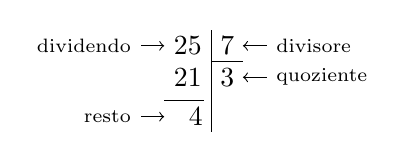
\begin{tikzpicture}

\draw[-](0,.4)--(0,-.9); % verticale
\draw[-](0,0)--(.4,0) ; %orizzontale
\draw (-.1,-.5) -- (-.6,-.5); % resto

\node (a) at (.2,.2) {7};
\node (b) at (.2,-.2) {3};
\node (c) at (-.3,.2) {25};
\node (d) at (-.3,-.2) {21};
\node (e) at (-.2,-.7){4};

\begin{scope}[font=\scriptsize]
  \draw  [<-] (.4,.2)--(.7,.2) node[right] {divisore};
  \draw  [<-] (.4,-.2)--(.7,-.2) node[right] {quoziente};
  \draw  [<-] (-.6,.2)--(-.9,.2) node[left] {dividendo};
  \draw  [<-] (-.6,-.7)--(-.9,-.7) node[left] {resto};
\end{scope}

\end{tikzpicture}

\end{center}

 \end{esempio}

 \begin{esempio}
 $0:2 =~0$.
 \end{esempio}

 \begin{esempio}
$1:2 =~0$ con resto~1.
 \end{esempio}

 \begin{esempio}
$5:2 =~2$ con resto~1.
 \end{esempio}
\end{exrig}

\osservazione Nella definizione di quoziente abbiamo sempre richiesto che il divisore sia diverso da zero. In effetti, se il divisore è~0 non c'è nessun numero che moltiplicato per~0 ci possa dare un dividendo diverso da zero.
Per esempio, nella divisione~$5:0$ dobbiamo ottenere un numero che moltiplicato per~0 dia~5; ciò non è
possibile in quanto qualsiasi numero moltiplicato per~0 dà~0.
Invece nella divisione~$0:0$ un qualsiasi numero è adatto come quoziente, infatti qualsiasi numero
moltiplicato per~0 dà~0 come prodotto.

Nel linguaggio matematico diciamo che una divisione del tipo~$n:0$, con~$n\neq~0$, è \emph{impossibile}; mentre la
divisione~$0:0$ è \emph{indeterminata}.

\begin{definizione}
 Dati due numeri naturali~$n$ e~$m$, con~$m\neq~0$, la \emph{divisione intera} tra $n$ e $m$ è l'operazione
che associa il più grande numero naturale~$q$ (il quoziente) per il quale si ha~$q\cdot m\le n$.
\end{definizione}

La divisione intera si indica con ``$\divint$'':
\begin{empheq}[box=\fbox]{equation*}
n \divint m = q\quad\text{(con resto }r\text{)}.
\end{empheq}

\begin{exrig}
 \begin{esempio}
$0 \divint 5=0$.
 \end{esempio}

 \begin{esempio}
$9 \divint 2=4$.
 \end{esempio}

 \begin{esempio}
$3\divint 5=0$.
 \end{esempio}

 \begin{esempio}
$3\divint 0 = $ non si può fare: la divisione intera per~0 non è possibile. 
 \end{esempio}
\end{exrig}

\begin{definizione}
 Dati due numeri naturali~$n$ e~$m$, con~$m\neq~0$, l'operazione che restituisce il resto della
divisione intera tra~$n$ e~$m$ si chiama \emph{modulo} di~$n$ rispetto a~$m$.
\end{definizione}

L'operazione di modulo viene indicata con ``$\bmod$'':
\begin{empheq}[box=\fbox]{equation*}
n\bmod{m} = r\quad\text{(dove }r\text{ è il resto di~~}n\divint m\text{)}.
\end{empheq}

\begin{exrig}
 \begin{esempio}
$0\bmod 5=0$.
 \end{esempio}

 \begin{esempio}
$9\bmod 5 =1$.
 \end{esempio}

 \begin{esempio}
$10\bmod 5=0$.
 \end{esempio}

 \begin{esempio}
$3\bmod 5=3$.
 \end{esempio}

 \begin{esempio}
$11\bmod 5=1$.
 \end{esempio}

 \begin{esempio}
$3\bmod 0=$ non si può fare.
 \end{esempio}
\end{exrig}

\ovalbox{\risolvii \ref{ese:1.2}, \ref{ese:1.3}, \ref{ese:1.4}, \ref{ese:1.5}, \ref{ese:1.6}}\vspazio

Ripassiamo l'algoritmo della divisione intera per numeri a più cifre; questa procedura risulterà particolarmente
utile nel seguito.

\begin{center}
 % (c) 2012 Dimitrios Vrettos - d.vrettos@gmail.com
\usetikzlibrary{matrix}

\begin{tikzpicture}
	\begin{scope}[every node/.style={anchor=base,row sep=1pt, column sep =-1pt, text depth=0pt, text height=6pt,text width=3pt}]%[font=\ttfamily]
 	\matrix (divisione) [matrix of nodes]
 	{%
 		&	3 & 2 & 7 &[.2cm] 2	&	3 &[.8cm] & 1 & 3 & 2 & 9 &[.2cm] 1 & 0 & 7 &[.8cm]   & 1 & 2	& 5	& 9 & 4 & 3 &[.2cm] 1 & 7 & 1\\
 	 |[gray]| -	& 2 & 3 &  	& |[blue]|1 & |[blue]|4 &  			|[gray]| -& 1 & 0 & 7 &  	  & |[blue]|1 & |[blue]|2	  &  	  & |[gray]|- & 1 & 1 	& 9 & 7 &  	&  	& |[blue]|7 & |[blue]|3 & |[blue]|6\\
 	   	&   	& 9 & 7 &  	&  	& 			  &	  & 2 & 5 & 9 &  	  &		  &  	 &  &     &  & 6 & 2 & 4 &  &  &  & \\
       &|[gray]|-  & 9 & 2 &  &  &  &|[gray]|  - & 2 & 1 & 4 &  &  &  &  &     &|[gray]| - & 5 & 1 & 3 &  &  &  & \\
      &  &  & |[red]|5 &  &  &  &   &  & |[red]|4 & |[red]|5 &  &  &  &  &     &  & 1 & 1 & 1 & 3 &  &  & \\
	 &  &  &  &  &  &  &   &  &  &  &  &  &  &  &     & |[gray]|- & 1 & 0 & 2 & 6 &  &  & \\
	& & & & |[white]|- & & &  & & & & |[white]|- & & & &    & & & & |[red]|8 & |[red]| 7 & & & \\
 	};
	\end{scope}
	% Prima divisione
	\draw(divisione-1-5.north west)--(divisione-2-5.south west);
	\draw(divisione-1-5.south west)--(divisione-1-6.south east);
	\draw(divisione-2-2.south west)--(divisione-2-3.south east);
	\draw(divisione-4-3.south west)--(divisione-4-4.south east);
	% Seconda divisione
	\draw (divisione-1-12.north west) -- (divisione-2-12.south west);
	\draw (divisione-1-12.south west) -- (divisione-1-14.south east);
	\draw(divisione-2-8.south west)--(divisione-2-10.south east);
	\draw (divisione-4-9.south west) -- (divisione-4-11.south east);
	% Terza divisione
	\draw (divisione-1-22.north west) -- (divisione-2-22.south west);
	\draw (divisione-1-22.south west) -- (divisione-1-24.south east);
	\draw (divisione-2-16.south west) -- (divisione-2-19.south east);
	\draw (divisione-4-18.south west) -- (divisione-4-20.south east);
	\draw (divisione-6-18.south west) -- (divisione-6-21.south east);
	% Frecce
	\draw[densely dotted,->] (divisione-1-4) -- (divisione-3-4);
	\draw[densely dotted,->] (divisione-1-11) -- (divisione-3-11);
	\draw[densely dotted,->] (divisione-1-20) -- (divisione-3-20);
	\draw[densely dotted,->] (divisione-1-21) -- (divisione-5-21);
	% Didascalie
	\node (a) [below=of divisione-7-5.north west] {(a)};
	\node (b) [below=of divisione-7-12.north west] {(b)};
	\node (c) [below=of divisione-7-21.north west] {(c)};
\end{tikzpicture}

\end{center}

\begin{enumeratea}
 \item $327:23=$ quoziente~14 e resto~5;
 \item $1\,329:107=$ quoziente~12 e resto~45;
 \item $125\,943:171=$ quoziente~736 e resto~87.
\end{enumeratea}

\ovalbox{\risolvi \ref{ese:1.7}}

\section{Proprietà delle operazioni}

\subsection{Proprietà commutativa}
Un'operazione ($\diamond$) gode della proprietà \emph{commutativa} se, cambiando l'ordine dei numeri sui quali essa va
eseguita, il risultato non cambia.

\begin{empheq}[box=\fbox]{equation*}
a\diamond b = b\diamond a.
\end{empheq}

La proprietà commutativa \emph{vale} per le seguenti operazioni:
\begin{description*}
 \item[addizione]~$a+b=b+a$. \quad Es.~$3+5=5+3=8$;
 \item[moltiplicazione]~$a\cdot b=b\cdot a$. \quad Es.~$3\cdot 5=5\cdot 3=15$.
\end{description*}

La proprietà commutativa \emph{non vale} per le seguenti operazioni:
\begin{description*}
 \item[sottrazione]~$a-b\neq b-a$. \quad Es.~$8-3=5\neq 3-8\:\text{ non si può fare in }\insN$;
 \item[divisione]~$a:b\neq b:a$. \quad Es.~$8:4=2\neq 4:8\:\text{ non si può fare in }\insN$;
 \item[divisione intera]~$a\divint b\neq b\divint a$. \quad Es.~$17\divint~5=3\neq~5\divint~17=0$;
 \item[modulo]~$a\bmod b\neq b\bmod a$. \quad Es.~$9\bmod~2=1\neq~2\bmod~9=2$;
 \item[potenza]~$a^b\neq b^a$. \quad Es.~$3^2=9\neq~2^3=8$.
\end{description*}

\subsection{Proprietà associativa}
Un'operazione ($\diamond$) gode della proprietà \emph{associativa} se, presi arbitrariamente tre numeri legati da due operazioni,
è indifferente da quale operazione si inizia, in quanto il risultato che si ottiene è sempre lo stesso.

\begin{empheq}[box=\fbox]{equation*}
(a\diamond b) \diamond c = a\diamond (b \diamond c).
\end{empheq}

La proprietà associativa \emph{vale} per le seguenti operazioni:
\begin{description*}
 \item[addizione]~$(a+b)+c=a+(b+c)$. \quad Es.~$(3+5)+2=3+(5+2)=10$;
 \item[moltiplicazione]~$(a\cdot b)\cdot c=a\cdot (b\cdot c)$. \quad Es.~$(3\cdot 5)\cdot 2=~3\cdot(5\cdot 2)=30$.
\end{description*}

La proprietà associativa \emph{non vale} per le seguenti operazioni:
\begin{description*}
 \item[sottrazione]~$(a-b)-c\neq a-(b-c)$. \quad Es.~$(10-5)-2=3\neq~10-(5-2)=7$;
 \item[divisione]~$(a:b):c\neq a:(b:c)$. \quad Es.~$(16:4):2=2\neq~16:(4:2)=8$;
 \item[divisione intera]~$(a\divint b)\divint c\neq a\divint(b\divint c)$. \\\quad Es.~$(17\divint~5)\divint~2=1\neq~17	\divint%
			 (5\divint2)=8$;
 \item[modulo]~$(a\bmod b)\bmod c\neq a\bmod(b\bmod c)$. \\\qquad Es.~$(17\bmod~7)\bmod~1=1$~$\neq~17\bmod(7\bmod2)=0$.
\end{description*}

\subsection{Elemento neutro}
Un'operazione ($\diamond$) ha un \emph{elemento neutro} $n$ se composto con qualsiasi altro numero lo lascia invariato, sia quando
il numero è a destra, sia quando è a sinistra dell'operatore.

\begin{empheq}[box=\fbox]{equation*}
a\diamond n = n\diamond a = a.
\end{empheq}

L'elemento neutro dell'addizione è~0, sia che si trovi a destra che a sinistra:
\[a+0=~0+a =a.\]
L'elemento neutro della moltiplicazione è~1, sia che si trovi a destra sia che si trovi a sinistra:
\[a\cdot 1 =~1\cdot a = a.\]
La divisione ha l'elemento neutro a destra, che è~1, ma non ha elemento neutro a sinistra:
\[a:1 = a \quad~(1:a\neq a\text{, \:se }a\neq~1).\]
In maniera analoga, anche la sottrazione ha l'elemento neutro~0 solo a destra:
\[a-0 = a \quad~(0-a\neq a\text{, \:se }a\neq~0).\]

\subsection{Proprietà distributiva}

La proprietà \emph{distributiva} coinvolge due operazioni differenti ($\diamond$ e $\star$). La proprietà distributiva di $\star$ rispetto a $\diamond$ è espressa in simboli:

\begin{empheq}[box=\fbox]{align*}
a \star (b \diamond c) &= a \star b \diamond a \star c\\
(a \diamond b) \star c &= a \star c \diamond b \star c.
\end{empheq}

\subsubsection{Proprietà distributiva della moltiplicazione}
\paragraph{Rispetto all'addizione}
Moltiplicare il risultato dell'addizione di più numeri per un altro numero dà lo stesso risultato che
moltiplicare ogni addendo per il fattore considerato e addizionare i prodotti ottenuti. Questa proprietà vale sia se la somma è a destra sia se è a sinistra.
\begin{flalign*}
 a\cdot(b+c) = a\cdot b +a\cdot c &\text{\quad Es.~}3\cdot(2+4) = 3\cdot 2+3\cdot 4=18\\
 (a+b)\cdot c = a\cdot c + b\cdot c &\text{\quad Es.~}(2+4)\cdot 3 = 2\cdot 3 + 4\cdot 3=18.
\end{flalign*}

\paragraph{Rispetto alla sottrazione}
In maniera analoga:
\begin{flalign*}
 a\cdot(b-c) = a\cdot b -a\cdot c &\text{\quad Es.~}6\cdot(10-4) = 6\cdot 10-6\cdot 4=36\\
 (a-b)\cdot c = a\cdot c - b\cdot c &\text{\quad Es.~}(10-4)\cdot 6 = 10\cdot 6- 4\cdot 6=36.
\end{flalign*}

\subsubsection{Proprietà distributiva della divisione}
\paragraph{Rispetto all'addizione}
Solo se le somme sono a sinistra:
\begin{flalign*}
 (a+b+c):d=a:d+b:d+c:d &\text{\quad Es.~}(20+10+5):5=20:5+10:5+5:5=7.
\end{flalign*}

Verifichiamo con un esempio che non vale la proprietà distributiva se le somme si trovano a destra:~$120:(3+5)$
Eseguendo prima l'operazione tra parentesi si ottiene correttamente~$120:8=15$. Se si prova ad applicare
la proprietà distributiva si ottiene~$120:3+120:5=40+24=64$. Il risultato corretto è il primo.

\paragraph{Rispetto alla sottrazione}
Solo se la sottrazione è a sinistra:
\begin{flalign*}
 (a-b):c=a:c-b:c &\text{\quad Es.~}(20-10):5=20:5-10:5=4-2=2.
\end{flalign*}

Se, però, la sottrazione è a destra:
\[120:(5-3)=120:2=60\neq~120:5-120:3=24-40=\:\text{ non si può fare in }\insN.\]

\begin{legge}[Annullamento del Prodotto]\label{legge:annullamento_del_prodotto}
 Il prodotto di due o più numeri naturali si annulla se e solo se almeno uno dei fattori è nullo.
%\[ a\cdot b=0\quad\Leftrightarrow\quad a=0\,\text{ oppure }\,b=0. \]
\end{legge}
In simboli:
\begin{empheq}[box=\fbox]{equation*}
a\cdot b=0\quad\Leftrightarrow\quad a=0\;\vee\;b=0.
\end{empheq}

\begin{proof}
La dimostrazione verrà fatta prima per l'implicazione diretta ($\Rightarrow$) e poi per quella inversa ($\Leftarrow$).
\begin{enumerate}
\item $a\cdot b = 0 \:\Rightarrow\: a = 0\;\vee\;b=0$~~si dimostra per assurdo.

Supponiamo che esistano due valori $a$ e $b$ entrambi non nulli, per i quali vale la condizione $a\cdot b = 0$. Poiché $b\neq 0$ possiamo dividere per $b$ le quantità a destra e a sinistra del simbolo di uguaglianza, mantenendo comunque verificata l'uguaglianza stessa. Quindi abbiamo $a\cdot b : b = 0 : b$. Visto che $(a\cdot b):c = a\cdot(b:c)$ e che qualunque numero diviso se stesso da come risultato 1, la parte a sinistra del simbolo disuguaglianza è $a \cdot b : b = a \cdot 1 = a$. Poiché 0 diviso qualunque numero diverso da zero dà come risultato 0, la parte a destra dell'uguaglianza vale $0 : b = 0$. Dunque mettendo insieme i passaggi precedenti otteniamo $a = 0$, che contraddice l'ipotesi iniziale ($a$ e $b$ entrambi non nulli), cioè siamo arrivati ad un assurdo. Pertanto abbiamo dimostrato che $a\cdot b = 0 \:\Rightarrow\: a = 0\;\vee\;b=0$.

\item La dimostrazione dell'implicazione inversa ($a = 0\;\vee\;b=0 \:\Rightarrow\: a\cdot b = 0$) è banale e deriva direttamente dalla definizione dell'operazione di moltiplicazione. Infatti se $a = 0$ qualunque sia $b$ si ha $0\cdot b = 0$. Lo stesso ragionamento vale per $b=0$.
\end{enumerate}
\end{proof}

%questo è presente anche nella prima pagina del capitolo 14
Il matematico Carl Friedrich Gauss\footnote{matematico, astronomo e fisico tedesco (1777 - 1855).} fu un bambino prodigio. Si racconta che a nove anni il suo insegnante ordinò di fare la somma dei numeri da~$1$~a~$100$. Poco dopo Gauss diede la risposta esatta sorprendendo il suo insegnante. Probabilmente egli aveva scritto in una riga i numeri da~$1$~a~$100$ e nella riga sottostante i numeri da~$100$~a~$1$, notando che ogni colonna dava per somma $101$. Quindi, anziché sommare uno ad uno i numeri da 1 a 100, moltiplicando $100$ per $101$ e dividendo il risultato per~$2$ Gauss aveva ottenuto rapidamente la risposta: $100 \cdot 101 : 2=\np{5050}$.
\begin{center}
\begin{tabular*}{.75\textwidth}{@{\extracolsep{\fill}}*{10}{r}}
$1$&$2$&$3$&$4$&$5$&$\ldots$&$97$&$98$&$99$&$100$\\
$100$&$99$&$98$&$97$&$96$&$\ldots$&$4$&$3$&$2$&$1$\\
\midrule
$101$&$101$&$101$&$101$&$101$&$\ldots$&$101$&$101$&$101$&$101$\\
\end{tabular*}
\end{center}

\ovalbox{\risolvii \ref{ese:1.8}, \ref{ese:1.9}}

\section{Potenza}\label{sect:potenza}
La \emph{potenza} di un numero naturale è una moltiplicazione che ha tutti i fattori uguali.

\begin{definizione}
Dati due numeri naturali~$a$ e~$n$, con~$n>1$, il primo detto \emph{base} ed il secondo \emph{esponente}, la potenza di~$a$ con esponente~$n$ è il numero~$p$ che si ottiene moltiplicando fra loro~$n$ fattori tutti uguali ad~$a$.
Si scrive~$a^n=p$ e si legge ``\emph{$a$ elevato a~$n$ uguale a~$p$}''.
\end{definizione}

Per esempio,~$5^3=5\cdot~5\cdot~5=125$.
\begin{center}
 % (c) 2012 Dimitrios Vrettos - d.vrettos@gmail.com
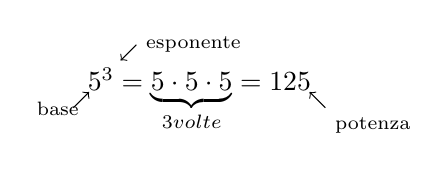
\begin{tikzpicture} 
  \node (esp) at (0,0) {$5^3=\underbrace{5\cdot 5\cdot 5}_{3 \text{ volte}} = 125$};
\begin{scope}[font=\scriptsize]
  \draw[<-]  (-1,.5)--(-0.8,.7) node[right] {esponente};
  \draw[->]  (-1.6,-.1)--(-1.4,.1) node[below left=.2] {base};
  \draw[<-]  (1.4,.1)--(1.6,-.1) node[below right] {potenza };
\end{scope}
\end{tikzpicture}

\end{center}

Quindi, in simboli
\begin{empheq}[box=\fbox]{equation*}
a^n = \underbrace{a\cdot a\cdot \ldots{} \cdot a}_{n \text{ volte}}
\end{empheq}

Per completezza, alla definizione precedente vanno aggiunti i seguenti casi particolari:
\begin{empheq}[box=\fbox]{align*}
 a^1&=a\text{,}\\
 a^0&=1\quad \text{se }a\neq~0\text{,}\\
 0^0&=\text{non ha significato.}
\end{empheq}

Queste definizioni trovano giustificazione nelle proprietà delle potenze.

\subsection{Proprietà delle potenze}

 \paragraph{I} Il prodotto di due potenze con la stessa base è uguale a una potenza che ha
 per base la stessa base e per esponente la somma degli esponenti.
 \begin{empheq}[box=\fbox]{equation*}
 a^n\cdot a^m=a^{n+m}
 \end{empheq}
 \[ 2^5\cdot 2^6=2^{5+6}=2^{11}.\]

La proprietà segue da questa osservazione:
\[ a^n\cdot a^m = \underbrace{(a\cdot a\cdot\ldots\cdot a)}_{n\text{ volte}}\cdot%
 \underbrace{(a\cdot a\cdot a\cdot\ldots\cdot a)}_{m\text{ volte}}
 =\underbrace{(a\cdot a\cdot a\cdot a\cdot a\cdot\ldots\cdot a\cdot a)}_{n+m\text{ volte}}%
 =a^{n+m}.\]

\paragraph{II} Il quoziente di due potenze con la stessa base, la prima con esponente
maggiore o uguale all'esponente della seconda, è uguale a una potenza che
ha per base la stessa base e per esponente la differenza degli esponenti.

 \begin{empheq}[box=\fbox]{equation*}
 a^n:a^m=a^{n-m}
 \end{empheq}
\[4^5:4^3=4^{5-3}=4^2.\]

La proprietà segue da questa osservazione:
\begin{align}
 a^n: a^m &= \underbrace{(a\cdot a\cdot\ldots\cdot a)}_{n\text{ volte}}:%
 \underbrace{(a\cdot a\cdot a\cdot\ldots\cdot a)}_{m\text{ volte}}\label{eq:pot_quoz1}\\
 &=\underbrace{(a:a)\cdot(a:a)\cdot\ldots\cdot(a:a)}_{n\text{ volte}}\cdot%
 \underbrace{(a\cdot a\cdot a\cdot\ldots\cdot a)}_{n-m\text{ volte}}\label{eq:pot_quoz2}\\%
 &=a^{n-m}.
\end{align}
Il passaggio dalla \ref{eq:pot_quoz1} alla \ref{eq:pot_quoz2} avviene per via della proprietà invariantiva della divisione.
\paragraph{III} La potenza di una potenza è uguale a una potenza che ha la base della prima
potenza e per esponente il prodotto degli esponenti.

 \begin{empheq}[box=\fbox]{equation*}
 (a^n)^m=a^{n\cdot m}
 \end{empheq}
\[(6^2)^5=6^{2\cdot 5}=6^{10}. \]

La proprietà segue da questa osservazione:

\[ (a^n)^m =\overbrace{a^n\cdot a^n\cdot\ldots\cdot a^n}^{m\text{ volte}}%
 =\overbrace{\underbrace{(a\cdot a\cdot\ldots\cdot a)}_{n\text{ volte}}\cdot%
	 \underbrace{(a\cdot a\cdot\ldots\cdot a)}_{n\text{ volte}}\cdot\ldots\cdot%
	 \underbrace{(a\cdot a\cdot\ldots\cdot a)}_{n\text{ volte}}}^{m\text{ volte}}%
	 =a^{n\cdot m}.\]

\paragraph{IV} Il prodotto di potenze con lo stesso esponente è
uguale al prodotto delle potenze dei singoli fattori.

 \begin{empheq}[box=\fbox]{equation*}
 (a\cdot b)^n=a^n\cdot b^n
 \end{empheq}
\[(2\cdot 5)^8=2^8\cdot 5^8. \]

La proprietà segue da questa osservazione:
\[(a\cdot b)^n=\underbrace{(a\cdot b)\cdot(a\cdot b)\cdot\ldots\cdot(a\cdot b)}_{n\text{ volte}}%
	 =\underbrace{(a\cdot a\cdot\ldots\cdot a)}_{n\text{ volte}}\cdot%
	 \underbrace{(b\cdot b\cdot\ldots\cdot b)}_{n\text{ volte}}%
	 =a^n\cdot b^n.\]

\paragraph{V} La potenza di un quoziente è uguale al quoziente delle potenze dei singoli
fattori.

 \begin{empheq}[box=\fbox]{equation*}
 (a:b)^n=a^n:b^n
 \end{empheq}
\[(4:2)^8=4^8:2^8. \]

Le definizioni dei casi particolari di potenze si giustificano nel seguente modo:
\begin{align*}
 &a^0=a^{5-5}=a^5:a^5=1,\\
 &a^1=a^{5-4}=a^5:a^4=a.
\end{align*}
Alla potenza~$0^0$ non si assegna nessun valore perché applicando la definizione di~$a^0$ si dovrebbe avere~1;
applicando la definizione~$0^a$ si dovrebbe avere~0.

\ovalbox{\risolvii \ref{ese:1.10}, \ref{ese:1.11}, \ref{ese:1.12}, \ref{ese:1.13}, \ref{ese:1.14}}\vspazio

\subsection{Cenni sull'estrazione di radice}

L'operazione inversa dell'elevazione a potenza è l'estrazione di \emph{radice}.

\begin{definizione}
Dati due numeri naturali~$a$ e~$n$ (con~$n>1$) si definisce \emph{radice}~$n$-esima di~$a$ il numero~$r$ tale che moltiplicando tra loro~$n$ fattori tutti uguali a~$r$ si ottiene come risultato~$a$.
\end{definizione}

In simboli:
\begin{empheq}[box=\fbox]{equation*}
\sqrt[n]{a} = r.%\quad\text{se}\quad r^n=a.
\end{empheq}

Per esempio~$\sqrt[3]{64} = 4$ poiché $4^3=4\cdot 4\cdot 4 = 64$.

\begin{exrig}
 \begin{esempio}
$\sqrt[5]{32} = 2$,~~infatti $2^5 = 2\cdot 2\cdot 2\cdot 2\cdot 2 = 32$.
 \end{esempio}

 \begin{esempio}
$\sqrt[3]{125} = 5$,~~infatti $5^3 = 5\cdot 5\cdot 5 = 125$.
 \end{esempio}

 \begin{esempio}
$\sqrt[4]{81} = 3$,~~infatti $3^4 = 3\cdot 3\cdot 3\cdot 3 = 81$.
 \end{esempio}

 \begin{esempio}
$\sqrt[7]{1} = 1$,~~infatti $1^7 = 1\cdot 1\cdot 1\cdot 1\cdot 1\cdot 1\cdot 1 = 1$.
 \end{esempio}
\end{exrig}

Particolare importanza riveste la radice con $n=2$, detta anche \emph{radice quadrata}. Ad esempio, la radice quadrata di 25 è 5, cioè $\sqrt[2]{25} = 5$, poiché infatti~$5^2 = 5\cdot 5=25$, e anche $\sqrt[2]{49} = 7$ ($7^2=49$). L'uso della radice quadrata è talmente predominante in matematica rispetto a quelle di ordine superiore (quelle con $n>2$) che nel caso in cui l'indice $n$ della radice non sia specificato si sottintende il valore 2: cioè $\sqrt{9} = \sqrt[2]{9} = 3$.


\section{Numeri Primi}

Osserva il seguente schema
\[\fbox{18}\quad\xrightarrow[\text{è divisibile per}]{\text{è multiplo di}}\quad \fcolorbox{gray}{grigio80}{6}\quad%
 \xrightarrow[\text{è divisore di}]{\text{è sottomultiplo di}}\quad \fbox{18}
\]
In esso sono descritte alcune caratteristiche del numero~18 e i suoi legami con il numero~6.

\begin{definizione}
 Chiamiamo \emph{divisore proprio} di un numero un suo divisore diverso dal numero stesso e dall'unità.
\end{definizione}

Osserva ora il seguente schema
\[\fbox{31}\quad\xrightarrow[\text{è divisibile per}]{\text{è multiplo di}}\quad \fcolorbox{gray}{grigio80}{\vphantom{3}\ldots}\quad%
 \xrightarrow[\text{è divisore di}]{\text{è sottomultiplo di}}\quad \fbox{31}
\]
Nella casella centrale, al posto dei puntini, puoi inserire soltanto i numeri~31 o~1.

\begin{definizione}
 Un numero~$p>1$ si dice \emph{primo} se è divisibile solo per se stesso e per l'unità. Un numero naturale maggiore di~1 non primo si dice \emph{composto}.
\end{definizione}

Per come sono stati definiti i numeri primi e quelli composti si ha:

\begin{multicols}{3}
\noindent~0 non è primo né composto;\\
1 non è primo né composto;\\
2 è primo;\\
3 è primo;\\
4 è composto;\\
5 è primo;\\
6 è composto;\\
7 è primo;\\
8 è composto;\\
9 è composto;\\
10 è composto;\\
11 è primo;\\
12 è composto;\\
13 è primo.\\
\ldots
\end{multicols}

\begin{exrig}
 \begin{esempio}
 Per verificare se~31 è primo, calcolo il valore approssimato~$\sqrt{31}\simeq\np{5,5}$ e verifico se è divisibile
per i numeri primi~$\le5$, cioè~2,~3 e~5. 31 non è divisibile per~2 in
quanto è dispari, non è divisibile per~3 poiché la somma delle sue cifre è~4 (che non è divisibile per~3) e
non è divisibile per~5 in quanto non finisce per~0 o~5 (sezione \ref{sect:criteri_divisibilita}). Quindi 31 è primo.
 \end{esempio}

 \begin{esempio}
 Per verificare se~59 è un numero primo calcolo~$\sqrt{59}\simeq\np{7,6}$ e verifico se~59 è divisibile per un
numero primo~$\le~7$, cioè per~2,~3,~5 e~7. Eseguendo le divisioni si vede che~59 non è divisibile
per nessuno di questi numeri, quindi è primo.
 \end{esempio}
\end{exrig}

\osservazione Un numero è primo quando non è divisibile per nessun numero primo compreso tra~2 e
la radice quadrata del numero stesso.

\vspazio\ovalbox{\risolvii \ref{ese:1.15}, \ref{ese:1.16}}


\section{Criteri di divisibilità}\label{sect:criteri_divisibilita}

Per verificare se un numero è divisibile per i primi numeri interi si possono applicare i seguenti criteri di
divisibilità.

\paragraph{Divisibilità per~2} Un numero è divisibile per~2 se e solo se la sua ultima cifra, quella delle unità,
è un numero pari, cioè è~0,~2,~4,~6,~8.

\begin{itemize*}
 \item \np{1236} finisce per~6 quindi è divisibile per~2;
 \item \np{109230} finisce per~0 quindi è divisibile per~2;
 \item \np{10923} finisce per~3 quindi non è divisibile per~2.
\end{itemize*}

\paragraph{Divisibilità per~3} Un numero è divisibile per~3 se e solo se la somma delle cifre che lo
compongono è divisibile per~3.
\begin{itemize*}
 \item 24 è divisibile per~3, infatti la somma delle sue cifre è~$2+4=6$, dato che~6 è divisibile per~3
anche~24 è divisibile per~3;
 \item \np{1236} è divisibile per~3, infatti la somma delle sue cifre è~$1+2+3+6=12$;~12~è divisibile per~3
dato che la somma delle sue cifre è~$1+2=3$, quindi anche~\np{1236} è divisibile per~3;
 \item 31 non è divisibile per~3, infatti la somma delle sue cifre è~$3+1=4$, dato che~4 non è
divisibile per~3 neanche~31 è divisibile per~3.
\end{itemize*}

\paragraph{Divisibilità per~5} Un numero è divisibile per~5 se la sua ultima cifra è~0 o~5.
\begin{itemize*}
 \item \np{1230} finisce per~0 quindi è divisibile per~5;
 \item \np{59235} finisce per~5 quindi è divisibile per~5;
 \item \np{109253} finisce per~3 quindi non è divisibile per~5;
 \item \np{5556} finisce per~6 quindi non è divisibile per~5.
\end{itemize*}

\paragraph{Divisibilità per~7} Un numero (maggiore di~10) è divisibile per~7 se la differenza (in valore assoluto\footnote{il \emph{valore assoluto} è trattato a pagina~\pageref{def:valass}.})
fra il valore ottenuto dal numero stesso togliendo la cifra delle unità e il doppio della cifra delle unità è~7 o un
multiplo di~7.
\begin{itemize*}
 \item 252 è divisibile per~7, infatti~$ \valass{25−2\cdot 2}=21$ è multiplo di~7;
 \item 49 è divisibile per~7, infatti~$\valass{4−2\cdot 9}=14$ è multiplo di~7;
 \item 887 non è divisibile per~7, infatti~$\valass{88−2\cdot 7}=74$ non è divisibile per~7.
\end{itemize*}

\paragraph{Divisibilità per~11} Un numero è divisibile per~11 se e solo se la differenza, in valore assoluto, fra la
somma delle cifre di posto pari e la somma delle cifre di posto dispari è~0,~11~o un multiplo di~11.
\begin{itemize*}
 \item 253 è divisibile per~11, infatti~$\valass{5-(2+3)}=0$;
 \item \np{9482} è divisibile per~11, infatti~$\valass{(9+8)−(4+2)}=11$;
 \item 887 non è divisibile per~11, infatti~$\valass{8-(8+7)}=7$.
\end{itemize*}

\ovalbox{\risolvii \ref{ese:1.17}, \ref{ese:1.18}}


\section{Scomposizione in fattori primi}

Scomporre in fattori (o fattorizzare) un numero significa scriverlo come prodotto di altri numeri naturali.

\begin{teorema}[fondamentale dell'aritmetica]\label{th:fondamentale_dell_aritmetica}
 Ogni numero naturale~$n>1$ si può scrivere in modo unico come prodotto di numeri primi.
\end{teorema}

%\begin{proof}
%La dimostrazione sarà effettuata in più fasi. Dapprima (punti 1 e 2) procederemo col dimostrare la possibilità di scrivere un numero sotto forma di prodotto di numeri primi (fattorizzazione). Quindi (punto 3) dimostreremo che tale fattorizzazione è unica.
%
%\begin{enumerate}
%\item \emph{Dimostriamo per induzione che ogni numero è divisibile per un numero primo o è primo esso stesso.}
%
%Il numero 2 è primo. Supponiamo che ogni numero da 2 a $n$ sia primo o divisibile per un numero primo e dimostriamolo per $n+1$.
%
%Considerando $n+1$ si hanno due possibilità:
%\begin{itemize*}
%\item $n+1$ è primo.
%\item $n+1$ non è primo, quindi è divisibile per un numero $a$ compreso tra 2 e $n$, e per l'ipotesi induttiva o $a$ è primo oppure è divisibile per un numero primo $p$. Quindi lo sarà anche $n+1$.
%\end{itemize*}
%Pertanto $n+1$ è divisibile per un numero primo o è esso stesso un numero primo.
%
%\item \emph{Dimostriamo per induzione che ogni numero è scomponibile in fattori primi.}
%
%Il numero 2 è già banalmente fattorizzato. Supponiamo che ogni numero da 2 a $n$ si possa scrivere come prodotto di numeri primi e dimostriamo che questo vale anche per $n+1$.
%
%Considerando $n+1$ si hanno due possibilità:
%\begin{itemize*}
%\item $n+1$ è primo, quindi già fattorizzato.
%\item $n+1$ non è primo, quindi divisibile per un primo $p$ (per quanto dimostrato al punto 1). Si consideri il numero $m=(n+1):p$ che è minore di $n+1$ e quindi, per l'ipotesi induttiva, può essere scomposto in un prodotto di numeri primi e pertanto lo è anche $n+1=m\cdot p$.
%\end{itemize*}
%
%Dunque, ogni numero è scomponibile in fattori primi.
%
%\item \emph{Dimostriamo adesso, per assurdo, che se un numero ammette una scomposizione in fattori primi questa è unica.}
%
%Si supponga che esistano dei numeri scomponibili in fattori primi in più di un modo. Sia $m$ il numero più piccolo tra essi. Siano inoltre (\ref{eq:num_primi_scomp1}) e (\ref{eq:num_primi_scomp2}) due sue diverse fattorizzazioni
%
%\begin{equation}\label{eq:num_primi_scomp1}
%m = p_1 \cdot p_2 \cdot \ldots \cdot p_s
%\end{equation}
%\begin{equation}\label{eq:num_primi_scomp2}
%m = q_1 \cdot q_2 \cdot \ldots \cdot q_t
%\end{equation}
%
%\noindent dove i numeri $p_1$,\ldots,$p_s$ e $q_1$,\ldots,$q_t$ sono primi ma differenti tra loro, ovvero $\forall i,j \; p_i \neq q_j$ (se ci fosse un fattore primo $p_h=q_k$ potremmo dividere $m$ per tale fattore ottenendo così un numero $m' < m$ che avrebbe anch'esso due fattorizzazioni distinte, riconducendoci così al caso considerato), sebbene all'interno di ogni fattorizzazione possano comunque essere presenti fattori ripetuti.
%Dunque $p_1\neq q_1$ e, senza perdita di generalità, possiamo supporre che $p_1 < q_1$.
%
%Sia
%\begin{equation}\label{eq:num_primi_scomp3}
%n = (q_1-p_1)\cdot q_2 \cdot \ldots \cdot q_t.
%\end{equation}
%Si ha $n < m$ dato che, per la proprietà distributiva della moltiplicazione rispetto all'addizione, l'uguaglianza precedente si può scrivere come
%\begin{equation}\label{eq:num_primi_scomp4}
%n = q_1\cdot q_2\cdot \ldots \cdot q_t - p_1\cdot q_2\cdot \ldots\cdot q_t = m - p_1\cdot q_2\cdot \ldots \cdot q_t < m.
%\end{equation}
%
%Se il primo fattore di $n$, $q_1-p_1$, non fosse primo lo potremo fattorizzare ottenendo così una nuova fattorizzazione di $n$ che non ammetterebbe $p_1$ tra i suoi fattori. Infatti, per quanto ipotizzato precedentemente, $p_1$ è diverso da $q_1$, $q_2$, \ldots, $q_t$, inoltre esso non può comparire nell'eventuale fattorizzazione di $q_1-p_1$, poiché se ciò accadesse significherebbe che $q_1$ è divisibile per $p_1$ (infatti $q_1-p_1= p_1\cdot a \:\Rightarrow\: q_1 = p_1\cdot(1+a)$), il che non è possibile in quanto per ipotesi $q_1$ è un numero primo. Dunque $q_1-p_1$ è primo.
%
%Considerando l'ultima uguaglianza della (\ref{eq:num_primi_scomp4}) e sostituendo in essa $m$ con la (\ref{eq:num_primi_scomp1}) otteniamo
%
%\begin{equation}\label{eq:num_primi_scomp5}
%n= p_1 \cdot p_2 \cdot \ldots\cdot p_s-p_1\cdot q_2 \cdot \ldots \cdot q_t \:\Rightarrow\: n = p_1\cdot(p_2\cdot \ldots \cdot p_s- q_2\cdot \ldots\cdot q_t)
%\end{equation}
%
%In qualunque modo sia scomponibile il secondo fattore della (\ref{eq:num_primi_scomp5}), si ha una fattorizzazione di $n<m$ che contiene $p_1$ e che è quindi diversa da quella della (\ref{eq:num_primi_scomp3}), contrariamente all'ipotesi che $m$ sia il numero più piccolo che ammette più di una fattorizzazione.
%\end{enumerate}
%Dunque la scomposizione di un numero in fattori primi è unica.
%\end{proof}

\begin{exrig}
 \begin{esempio}
 Scomporre in fattori primi il numero~630.
 \begin{center}
% % (c) 2012 Dimitrios Vrettos - d.vrettos@gmail.com
\begin{tikzpicture}
\begin{scope}[font=\ttfamily]
\matrix (scomposizione)[matrix of nodes]{
	6&3&0 & 2\\
	3&1&5 & 3\\
	1&0&5 & 3\\
	&3&5 &5\\
	&&7 & 7\\
	&&1 & \\
};
\end{scope}
 \draw(scomposizione-1-3.north east)--(scomposizione-6-3.south east);

\node (a) [right=of scomposizione-1-4.east] {630 \`e divisibile per 2 perch\'e l'ultima cifra \`e pari;};
\node (b) [right=of scomposizione-2-4.east] {315 \`e divisibile per 3, la somma delle sue cifre \`e 9 divisibile per 3;};
\node (c) [right=of scomposizione-3-4.east] {105 \`e divisibile per 3, la somma delle sue cifre \`e 6 divisibile per 3;};
\node (d) [right=of scomposizione-4-4.east] {35 \`e divisibile per 5 perch\'e l'ultima cifra \`e 5;};
\node (e) [right=of scomposizione-5-4.east] {7 \`e un numero primo.};
\end{tikzpicture}

 \begin{tabular}{r|l@{\hspace{15mm}}l}
 	630 & 2 & 630 è divisibile per 2 perché l'ultima cifra è pari;\\
	315 & 3 & 315 è divisibile per 3 (la somma delle sue cifre è 9, divisibile per 3);\\
	105 & 3 & 105 è divisibile per 3 (la somma delle sue cifre è 6, divisibile per 3);\\
	35 & 5 & 35 è divisibile per 5 perché l'ultima cifra è 5;\\
	7 & 7 & 7 è un numero primo.\\
	1 & \\
 \end{tabular}
 ~$630=2\cdot3^2\cdot5\cdot7.$
 \end{center}
 \end{esempio}
\end{exrig}

In generale, un numero può essere scomposto in fattori in più modi. Per esempio,~$12=3\cdot 4$,
ma anche~$12=6\cdot2$. Il teorema fondamentale dell'aritmetica ci assicura che, se si scompone un numero in fattori primi,
questa scomposizione è unica, a meno dell'ordine con cui si scrivono i fattori. Tornando all'esempio
precedente~$12=~2^2\cdot 3$ è l'unico modo in cui il~12 si può scomporre in fattori primi, a meno che non si
scambino di posto i fattori~$12=3\cdot 2^2$.

I numeri primi sono quindi i mattoni fondamentali dell'aritmetica, poiché gli altri numeri naturali possono essere ottenuti, in maniera univoca, come prodotto di primi.

Sebbene al crescere dei valori considerati i numeri primi diventino sempre più radi, essi sono comunque infiniti, come affermò Euclide\footnote{matematico e scienziato della Grecia antica (367 \aC{} ca. - 283 \aC).} con il seguente teorema che porta il suo nome:
\begin{teorema}[di Euclide]
I numeri primi sono infiniti.
\end{teorema}

\begin{proof}
Il teorema può essere dimostrato per assurdo.
Supponiamo infatti che i numeri primi siano un numero finito, cioè siano, ordinati dal più piccolo al più grande, $p_1$, $p_2$, \ldots{}, $p_n$. Si consideri il numero $a=p_1\cdot p_2\cdot \ldots{}\cdot p_n+1$. Per com'è stato scelto, $a$ non è divisibile per nessuno dei numeri $p_1$, $p_2$, \ldots{}, $p_n$ poiché la divisione per qualunque di essi darà sempre come resto 1. Quindi o $a$ è un numero primo maggiore di $p_n$ oppure, per il teorema fondamentale dell'aritmetica (pagina \pageref{th:fondamentale_dell_aritmetica}), è divisibile per un numero primo $p^*$ differente da $p_1$, $p_2$, \ldots{}, $p_n$. In entrambi i casi si ha una contraddizione con l'ipotesi iniziale, cioè che i numeri primi siano un numero finito, poiché per come è stato scelto, $a$ implica l'esistenza di un numero primo che non è nell'elenco ipotizzato $p_1$, $p_2$, \ldots, $p_n$. Quindi i numeri primi sono infiniti.
\end{proof}

\ovalbox{\risolvii \ref{ese:1.19}, \ref{ese:1.20}}
%\vspazio\ovalbox{\risolvi \ref{ese:1.17}}


\subsection{Numeri primi e crittografia}

Il problema legato alla scomposizione in fattori primi è di notevole interesse per i matematici, poiché non è ancora stato individuato un meccanismo che permette di stabilire se un numero sia primo o meno\footnote{si tratta della dimostrazione dell'ipotesi di Riemann, uno dei 7 \emph{Millennium problems} elencati il 24 maggio 2000, ovvero questioni matematiche ad oggi (2014) ancora non dimostrate (tranne una). Vista l'enorme difficoltà nel riuscire nell'intento, il Clay Mathematics Institute ha messo in palio un milione di dollari per la dimostrazione di ognuna di esse (v.~\url{http://it.wikipedia.org/wiki/Problemi_per_il_millennio}).}, se non quello di provare a dividerlo per tutti i numeri minori o uguali alla sua radice quadrata, procedura che diventa sempre più lunga man mano che le cifre che compongono il numero da verificare aumentano. Per questo motivo l'utilizzo di valori che siano il prodotto di numeri primi con un numero elevato di cifre è ciò che sta alla base della moderna crittografia, ovvero dei sistemi per la cifratura dei messaggi.

Consideriamo un semplice esempio che può chiarire come funziona il meccanismo di base per inviare messaggi segreti.

Alice deve inviare la sua password, la parola ``BACI'', a suo fratello Bruno. Alice trasforma la parola in numeri secondo la semplice regola A=1, B=2, C=3, I=9 (assegnando ad ogni lettera il numero cardinale corrispondente alla sua posizione nell'alfabeto). Il messaggio diventa così~$ \np{2139} $. Alice moltiplica questo numero per un numero primo ``segreto'' (che conosce solo lei) $\np{26417}$ e ottiene $\np{2139} \cdot \np{26417}=\np{56505963}$ e invia quest'ultimo numero a Bruno. Chiunque intercetti questo numero non è in grado di individuare la password in chiaro.

Quando Bruno riceve il numero $ \np{56505963} $ lo moltiplica per un suo numero primo ``segreto'' (che conosce solo lui) $\np{43969}$ ottenendo $\np{5650593} \cdot \np{43969}=\np{2484510687147}$ e lo invia nuovamente ad Alice.

Quando Alice riceve il numero lo divide per il suo numero primo $\np{2484510687147} : \np{26417} = \np{94049691}$ e quindi lo rispedisce a Bruno,
A questo punto Bruno divide il numero ricevuto per il suo numero primo segreto ottenendo $\np{94049691} : \np{43969} = \np{2139}$. Conoscendo il meccanismo di codifica (relazione tra i numeri e le lettere dell'alfabeto  2=B, 1=A, 3=C, 9=I) Bruno può dunque ricostruire la password ``BACI''.

In realtà, i sistemi per lo scambio di messaggi cifrati oggi utilizzati per mezzo dei computer si basano su meccanismi leggermente differenti che evitano il doppio invio di messaggi tra Alice e Bruno. I meccanismi sono essenzialmente due: il primo è detto \emph{a chiave simmetrica}, in cui sia Alice che Bruno condividono il numero segreto con il quale viene cifrato il messaggio e quindi entrambi possono codificarlo e decodificarlo autonomamente; il secondo, un po' più complesso ma che dà le stesse garanzie del doppio invio di messaggi (nessuna condivisione del numero segreto tra gli interlocutori), viene chiamato \emph{a chiave asimmetrica} e si basa sull'utilizzo di un numero segreto ed un numero pubblico da condividere con l'interlocutore.

Va comunque sottolineato il fatto che la robustezza del meccanismo di cifratura sta nella difficoltà intrinseca della fattorizzazione di numeri molto grandi. Ciò non significa che i messaggi rimarranno segreti per sempre: prima o poi saranno decifrati visto che la velocità di calcolo dei computer è sempre in aumento. Per cercare di rendere il processo di decifratura più arduo si possono scegliere chiavi di cifratura composte da numeri primi sempre più grandi.


\section{Massimo Comune Divisore e minimo comune multiplo}

\label{def:mcd}
\begin{definizione}
Il \emph{massimo comune divisore} di numeri naturali~$a$ e~$b$, indicato con~$\mcd(a\text{,~}b)$, è il
più grande tra tutti i divisori comuni ad~$a$ e~$b$.
\end{definizione}

Applicando la definizione, il massimo comune divisore tra~18 e~12 si ottiene prendendo tutti i divisori
di~18 e di~12:
\begin{center}
\begin{tabular}{rl}
divisori di 18: &18, 9, 6, 3, 2, 1;\\
divisori di 12: &12, 6, 4, 2, 1.\\
\end{tabular}
\end{center}
I divisori comuni sono~6,~2 e~1. Il più grande dei divisori comuni è~6, quindi $\mcd(18\text{,~}12)=6$.

%\begin{align*}
%\text{divisori di 18:} &\text{~}18\text{, }9\text{, }6\text{, }3\text{, }2\text{, }1;\\
%\text{divisori di 12:} &\text{~}12\text{, }6\text{, }4\text{, }2\text{, }1.
%\end{align*}

Per calcolare il massimo comune divisore di due o più numeri si può applicare la seguente procedura:
\begin{procedura}
Calcolo del~$\mcd$ di due o più numeri naturali:
\begin{enumeratea}
 \item si scompongono i numeri in fattori primi;
 \item si moltiplicano tra loro i fattori comuni, presi una sola volta e con il minore esponente.
\end{enumeratea}
\end{procedura}

\begin{exrig}
 \begin{esempio}
 Calcolare~$\mcd(60\text{,~}48\text{,~}36)$.

Si scompongono in fattori i singoli numeri~$60=2^2\cdot 3\cdot 5$,~$48=2^4\cdot 3$ e~$36 =2^2\cdot 3^2$.
I~fattori comuni sono~2 e~3; il~2 compare con l'esponente minimo~2 ed il~3 compare con esponente
minimo~1.

Pertanto~$\mcd(60\text{,~}48\text{,~}36)=2^2\cdot 3=12$.

 \end{esempio}

 \begin{esempio}
 Calcolare~$\mcd(60\text{,~}120\text{,~}90)$.

Si scompongono in fattori i singoli numeri~$60=2^2\cdot 3\cdot 5$,~$120=2^3\cdot 3\cdot 5$ e~$90=2\cdot 3^2\cdot 5$.
I~fattori in comune sono~2,~3 e~5. L'esponente minino è~1 per tutti.

Pertanto~$\mcd(60\text{,~}120\text{,~}90)=2\cdot 3\cdot 5=30$.
 \end{esempio}
\end{exrig}


\begin{definizione}
 Due numeri~$a$ e~$b$ si dicono \emph{primi tra loro} o \emph{coprimi} se~$\mcd(a\text{,~}b)=1$.
\end{definizione}

\pagebreak
\begin{exrig}
 \begin{esempio}
 Numeri primi tra loro:
 \begin{itemize*}
 \item 12 e~25 sono primi tra loro. Infatti il~$\mcd(12\text{,~}25)=1$ dato che nelle loro scomposizioni in
fattori non si hanno fattori comuni:~$12=2^2\cdot 3$ e~$25=5^2$;
 \item 35 e~16 sono primi tra loro. Infatti~$35=5\cdot 7$ e~$16=2^4$. I due numeri non hanno
divisori comuni, quindi il loro~$\mcd=1$;
 \item 11 e~19 sono primi tra loro infatti il~$\mcd(11\text{,~}19)=1$ dato che~11 e~19 sono entrambi numeri primi;
 \item 12 e~15 non sono primi tra di loro in quanto hanno~3 come divisore comune.
 \end{itemize*}
 \end{esempio}
\end{exrig}


\begin{definizione}
 Il \emph{minimo comune multiplo} di due numeri naturali~$a$ e~$b$ si indica con~$\mcm(a\text{,~}b)$ ed è il più
piccolo tra tutti i multipli comuni di~$a$ e di~$b$.
\end{definizione}

Per calcolare il minimo comune multiplo tra~6 e~15 applicando la definizione occorre calcolare i primi
multipli dei due numeri:
\begin{center}
\begin{tabular}{rl}
multipli di 6: & 6, 12, 18, 24, 30, 36, 42, 48, 54, 60, \ldots;\\
multipli di 15: & 15, 30, 45, 60, 75, 90, \ldots\\
\end{tabular}
\end{center}
Sono multipli comuni~30,~60,~90, \ldots Il più piccolo di essi è~30, ovvero $\mcm(6\text{,~}15)=30$.
%\begin{align*}
%\text{multipli di }6: & \qquad~6\text{, }12\text{, }18\text{, }24\text{, }30\text{, }36\text{, }42\text{, }48\text{, }54\text{, }60\text{, }\ldots; \\
%\text{multipli di }15: & \qquad~15\text{, }30\text{, }45\text{, }60\text{, }75\text{, }90\text{, }\ldots
%\end{align*}

Per calcolare il minimo comune multiplo tra due o più numeri si può applicare la seguente procedura:
\begin{procedura}
Calcolo del~$\mcm$ di due o più numeri naturali:
\begin{enumeratea}
 \item si scompongono i numeri in fattori primi;
 \item si moltiplicano tra loro i fattori comuni e non comuni, presi una sola volta, con il maggiore
esponente.
\end{enumeratea}
\end{procedura}

\begin{exrig}
 \begin{esempio}
 Calcolare il~$\mcm(60\text{,~}48\text{,~}36)$.

Scomponendo in fattori i numeri si ha~$60=2^2\cdot 3\cdot 5$,~$48=2^4\cdot 3$ e~$36=2^2\cdot 3^2$.
Tutti i fattori comuni e non comuni presi una sola volta con l'esponente più grande con cui
compaiono sono:~$2^4$, $3^2$ e~$5$.

Quindi il~$\mcm$ è~$2^4\cdot3^2\cdot5=720$.
 \end{esempio}

 \begin{esempio}
 Calcolare il~$\mcm(20\text{,~}24\text{,~}450)$.

Scomponendo in fattori si ha:~$20=2^2\cdot 5$,~$24=2^3\cdot 3$ e~$450 =~2\cdot 3^2\cdot 5^2$.
Moltiplicando i fattori comuni e non comuni con il massimo esponente si ha~$2^3\cdot 3^2\cdot 5^2=\np{1800}$.
 \end{esempio}

 \begin{esempio}
 Si vuole pavimentare una stanza a pianta rettangolare di~$315\;\unit{cm}$ per~$435\;\unit{cm}$ con mattonelle quadrate le
più grandi possibili, senza sprecarne alcuna. Quali sono le dimensioni delle mattonelle? Quante
mattonelle sono necessarie?

Poiché le mattonelle devono essere quadrate devono avere il lato tale che entri un numero intero di
volte sia nel~315 sia nel~435, pertanto la dimensione delle mattonelle deve essere un divisore comune
di~315 e di~435. Poiché è richiesto che le mattonelle siano quanto più grandi possibile, la dimensione
deve essere il massimo divisore comune.
% % (c) 2012 Dimitrios Vrettos - d.vrettos@gmail.com
\begin{tikzpicture}[node distance=20ex]
\begin{scope}[font=\ttfamily]
  \matrix(doppio)[matrix of nodes]{
    3&1&5&3&[3mm]4&3&5&3&\\
    1&0&5&3&1&4&5&5&\\
    &3&5&5&&2&9&2&9\\
    &&7&7&&&1&&\\
    &&1&&&&&&\\
  };
\end{scope}
  \draw (doppio-1-3.north east) -- (doppio-5-3.south east);
  \draw (doppio-1-7.north east) -- (doppio-4-7.south east);

\node (a)[below=of doppio-1-5.south east] {$315=3^2\cdot5\cdot7$};
\node (a)[below=of doppio-2-5.south east] {$435=3\cdot5\cdot29$};
\end{tikzpicture}

\begin{multicols}{2}
\begin{center}
\begin{tabular}{r|l@{\hspace{10mm}}r|l}
 	315 & 3 & 435 & 3\\
	105 & 3 & 145 & 5\\
	35 & 5 & 29 & 29\\
	7 & 7 & &\\
	1 & & &\\
\end{tabular}

$315=3^2\cdot5\cdot7$\\
$435=3\cdot5\cdot29$
\end{center}
 % (c) 2012 Dimitrios Vrettos - d.vrettos@gmail.com
\begin{tikzpicture}
  \begin{scope}[scale=1,every node/.style={minimum size=1cm},on grid]
    \draw[step=10mm, black, dashed] (0,0) grid (6,5);
    \fill[gray, opacity=.4] (5,4) rectangle (6,5);
    \draw[black,very thick] (0,0) rectangle (6,5);
  \end{scope} 
\end{tikzpicture}

\end{multicols}
La soluzione del problema è data quindi dal~$\mcd(315\text{,~}435)=3\cdot 5=15$. Le mattonelle devono avere il lato di~$15\;\unit{cm}$.
Ci vogliono~$435:15=29$ mattonelle per ricoprire il lato di~$435\;\unit{cm}$ e~$315:15=21$ mattonelle per ricoprire il lato
da~$315\;\unit{cm}$. In tutto occorrono~$29\cdot21=609$ mattonelle.
\end{esempio}
\end{exrig}

\ovalbox{\risolvii \ref{ese:1.21}, \ref{ese:1.22}, \ref{ese:1.23}, \ref{ese:1.24}, \ref{ese:1.25}, \ref{ese:1.26}}

\section{Espressioni numeriche}

Nel linguaggio comune alcune frasi possono risultare ambigue. Per esempio
<<Luca ha detto Mario è stato promosso>> può avere due significati diversi
a seconda di come si inserisce la punteggiatura:
scrivendo <<Luca, ha detto Mario, è stato promosso>> significa che è stato promosso Luca;
scrivendo <<Luca ha detto: Mario è stato promosso>> significa che è stato promosso Mario.

Anche nella matematica, quando abbiamo più operazioni da eseguire, dobbiamo chiarire l'ordine con
cui esse devono essere eseguire. Per esempio, l'espressione~$2+3\cdot 4$ può valere~14 oppure~20, infatti:
\begin{itemize*}
 \item eseguendo per prima la moltiplicazione si ha~$2+3\cdot 4=2+12=14$;
 \item eseguendo per prima l'addizione si ha~$2+3\cdot 4=5\cdot 4=20$.
\end{itemize*}

Per eliminare queste ambiguità sono state fissate alcune regole che bisogna rispettare
nell'esecuzione dei calcoli. Intanto diamo la seguente definizione:

\begin{definizione}
 Un'\emph{espressione aritmetica} è una successione di operazioni da eseguire su più numeri.
\end{definizione}

\subsection{Regole per semplificare le espressioni}
\paragraph {I} Se un'espressione contiene solo addizioni, le operazioni si possono eseguire
in qualsiasi ordine, grazie alla proprietà associativa dell'addizione.
\begin{exrig}
 \begin{esempio}
 Semplificare l'espressione $3+2+5$.
\begin{itemize*}
 \item $3+2+5=5+5=10$. In questo caso si sono eseguite le operazioni nell'ordine in cui compaiono;
 \item $3+2+5=3+7=10$. In questo caso si è eseguita per prima l'ultima addizione indicata. Il risultato ottenuto è lo stesso;
 \item $5+6+15=6+20=26$. In questo caso abbiamo applicato anche la proprietà commutativa.
\end{itemize*}
 \end{esempio}
\end{exrig}


\paragraph {II} Se un'espressione contiene solo moltiplicazioni, le operazioni si possono eseguire in qualsiasi
ordine, anche in questo caso grazie alla proprietà associativa della moltiplicazione.
\begin{exrig}
 \begin{esempio}
 Dovendo moltiplicare~$2\cdot 3\cdot 4$ si può procedere in più modi.
\begin{itemize*}
 \item $2\cdot 3\cdot 4=6\cdot 4=24$. In questo caso si è seguito l'ordine in cui compaiono;
 \item $2\cdot 3\cdot 4=2\cdot 12=24$. In questo caso si è seguito l'ordine opposto; il risultato è lo stesso.
\end{itemize*}
 \end{esempio}
\end{exrig}

\paragraph {III} Se un'espressione, senza parentesi, contiene più sottrazioni, si deve procedere eseguendole
nell'ordine in cui sono scritte, la sottrazione infatti non gode né della proprietà associativa né di quella
commutativa.
\begin{exrig}
 \begin{esempio}
 Semplificare l'espressione $10-6-1$.
\begin{itemize*}
 \item $10-6-1=4-1=2$;
 \item $10-6-1=10-5=5$, errato!
\end{itemize*}
 \end{esempio}
\end{exrig}

\paragraph {IV} Se un'espressione senza parentesi contiene solo addizioni e sottrazioni, le operazioni si devono
eseguire nell'ordine con cui sono scritte.
\begin{exrig}
 \begin{esempio}
 Semplificare l'espressione $12+6-5-1+2$.
 \[12+6-5-1+2=18-5-1+2=13-1+2=12+2=14.\]
 \end{esempio}
\end{exrig}

\paragraph {V} Se un'espressione senza parentesi contiene solo divisioni, le operazioni si devono eseguire
nell'ordine nel quale sono scritte.
\begin{exrig}
 \begin{esempio}
 Semplificare l'espressione $360:~12:~3$.
 \begin{itemize*}
 \item $360:12:3=30:3=10$;
 \item $360:12:3=360:4=90$, errato!
\end{itemize*}
 \end{esempio}
\end{exrig}

\paragraph {VI} Se un'espressione senza parentesi contiene addizioni, sottrazioni, moltiplicazioni, divisioni e
potenze, si eseguono prima le potenze, poi moltiplicazioni e divisioni, rispettando l'ordine con cui sono
scritte, e poi addizioni e sottrazioni, rispettando l'ordine.
\pagebreak
\begin{exrig}
 \begin{esempio}
Semplificare l'espressione $18:2:9+5^2-2\cdot3^2:3-1$.
 \begin{align*}
 18:2:9+5^2-2\cdot3^2:3-1&=18:2:9+25-2\cdot 9:3-1\\
			 &=9:9+25-18:3-1\\
			 &=1+25-6-1\\
			 &=26-6-1\\
			 &=20-1\\
 &=19.
 \end{align*}
 \end{esempio}
\end{exrig}

\paragraph {VII} Se l'espressione contiene una coppia di parentesi si devono eseguire prima le operazioni
racchiuse nelle parentesi, rispettando le regole precedenti; si eliminano poi le parentesi ottienendo
un'espressione senza parentesi alla quale devono essere applicate nuovamente le regole precedenti.
\begin{exrig}
 \begin{esempio}
Semplificare l'espressione $5\cdot(4+3^2-1)$.
 \begin{align*}
 5\cdot(4+3^2-1)&=5\cdot(4+9-1)\\
		 &=5\cdot(13-1)\\
		 &=5\cdot 12\\
		 &=60.
 \end{align*}
\end{esempio}
\end{exrig}


\paragraph{VIII} Se l'espressione contiene più ordini di parentesi, si eseguono per prima le operazioni racchiuse nelle parentesi più interne, rispettando le regole precedenti, si eliminano le parentesi e si procede considerando la nuova espressione. Se ci sono ancora delle parentesi si eseguono per prima le operazioni contenute nelle parentesi più interne, rispettando le regole precedenti, si eliminano le parentesi e si procede considerando la nuova espressione. E così via.

Per facilitare il riconoscimento dei livelli di parentesi, in genere si usano le parentesi tonde $($\ldots$)$ per il primo livello (quello più interno), le quadre $[$\ldots$]$ per il secondo livello e le graffe $\{$\ldots$\}$ per il terzo livello (quello più esterno).
L'uso di parentesi di diverso tipo rende visivamente più evidente l'ordine da seguire nelle operazioni, ma in un'espressione le parentesi possono anche essere soltanto tonde. Ciò accade, per esempio, quando si usano gli strumenti di calcolo elettronico come il computer e la calcolatrice.

\vspazio\ovalbox{\risolvi\ref{ese:1.27}}
\newpage

% (c) 2012 -2014 Dimitrios Vrettos - d.vrettos@gmail.com
% (c) 2014 Claudio Carboncini - claudio.carboncini@gmail.com
\section{Esercizi}
\subsection{Esercizi dei singoli paragrafi}
\subsubsection*{\thechapter.4 - Operazioni con i numeri naturali}

\begin{esercizio}
\label{ese:1.1}
Rispondi alle seguenti domande:
 \begin{enumeratea}
 \item Esiste il numero naturale che aggiunto a~3 dà come somma~6?
 \item Esiste il numero naturale che aggiunto a~12 dà come somma~7?
 \item Esiste il numero naturale che moltiplicato per~4 dà come prodotto~12?
 \item Esiste il numero naturale che moltiplicato per~5 dà come prodotto~11?
 \end{enumeratea}
\end{esercizio}

\begin{esercizio}
\label{ese:1.2}
 Inserisci il numero naturale mancante, se esiste:
\begin{multicols}{3}
\begin{enumeratea}
 \item $7-\ldots =1$;
 \item$3-3=\ldots~$;
 \item$5-6=\ldots~$;
 \item $3-\ldots =9$;
 \item$15:5=\ldots~$;
 \item$18:\ldots =3$;
 \item $\ldots:4=5$;
 \item$12:9=\ldots~$;
 \item$36\cdot\ldots =9$.
\end{enumeratea}
\end{multicols}
\end{esercizio}

\begin{esercizio}
\label{ese:1.3}
 Vero o falso?
\begin{multicols}{2}
\TabPositions{3.2cm}
\begin{enumeratea}
 \item $5:0=0$	\tab\qquad\boxV\qquad\boxF
 \item $0:5=0$	\tab\qquad\boxV\qquad\boxF
 \item $5:5=0$	\tab\qquad\boxV\qquad\boxF
 \item $1:0=1$	\tab\qquad\boxV\qquad\boxF
 \item $0:1=0$	\tab\qquad\boxV\qquad\boxF
 \item $0:0=0$	\tab\qquad\boxV\qquad\boxF
 \item $1:1=1$	\tab\qquad\boxV\qquad\boxF
 \item $1:5=1$	\tab\qquad\boxV\qquad\boxF
\end{enumeratea}
\end{multicols}
\end{esercizio}

\begin{esercizio}
\label{ese:1.4}
 Se è vero che~$p=n\cdot m$, quali affermazioni sono vere?
\begin{multicols}{2}
\TabPositions{3.2cm}
\begin{enumeratea}
 \item $p$ è multiplo di~$n$	\tab\qquad\boxV\qquad\boxF
 \item $p$ è multiplo di~$m$	\tab\qquad\boxV\qquad\boxF
 \item $m$ è multiplo di~$p$	\tab\qquad\boxV\qquad\boxF
 \item $m$ è multiplo di~$n$	\tab\qquad\boxV\qquad\boxF
 \item $p$ è divisibile per~$m$	\tab\qquad\boxV\qquad\boxF
 \item $m$ è divisibile per~$n$	\tab\qquad\boxV\qquad\boxF
 \item $p$ è divisore di~$m$	\tab\qquad\boxV\qquad\boxF
 \item $n$ è multiplo di~$m$	\tab\qquad\boxV\qquad\boxF
\end{enumeratea}
\end{multicols}
\end{esercizio}

\begin{esercizio}
\label{ese:1.5}
 Quali delle seguenti affermazioni sono vere?

\begin{multicols}{2}
\TabPositions{3.2cm}
 \begin{enumeratea}
 \item 6 è un divisore di~3 \tab\qquad\boxV\qquad\boxF
 \item 3 è un divisore di~6 \tab\qquad\boxV\qquad\boxF
 \item 8 è un multiplo di~2 \tab\qquad\boxV\qquad\boxF
 \item 5 è divisibile per~10 \tab\qquad\boxV\qquad\boxF
 \end{enumeratea}
\end{multicols}
\end{esercizio}

\begin{esercizio}
\label{ese:1.6}
 Esegui le seguenti operazioni:
\begin{multicols}{2}
 \begin{enumeratea}
 \item $18\divint 3=\ldots$;
 \item $18\bmod 3=\ldots$;
 \item $20\divint 3=\ldots$;
 \item $20\bmod 3=\ldots$;
 \item $185\divint 7=\ldots$;
 \item $185\bmod 7=\ldots$;
 \item $97\divint 5=\ldots$;
 \item $97\bmod 5=\ldots$;
 \item $240\divint 12=\ldots$;
 \item $240\bmod 12=\ldots$.
 \end{enumeratea}
\end{multicols}
\end{esercizio}

\pagebreak
\begin{esercizio}
\label{ese:1.7}
 Esegui le seguenti divisioni con numeri a più cifre, senza usare la calcolatrice.
\begin{multicols}{4}
 \begin{enumeratea}
 \item $311:22$;
 \item $429:37$;
 \item $512:31$;
 \item $629:43$;
 \item $755:53$;
 \item $894:61$;
 \item $968:45$;
 \item $991:13$;
 \item $\np{1232}:123$;
 \item $\np{2324}:107$;
 \item $\np{3435}:201$;
 \item $\np{4457}:96$;
 \item $\np{5567}:297$;
 \item $\np{6743}:311$;
 \item $\np{7879}:201$;
 \item $\np{8967}:44$;
 \item $\np{13455}:198$;
 \item $\np{22334}:212$;
 \item $\np{45647}:721$;
 \item $\np{67649}:128$.
 \end{enumeratea}
\end{multicols}
\end{esercizio}

\subsubsection*{\thechapter.5 - Proprietà delle operazioni}
\begin{esercizio}
\label{ese:1.8}
 Stabilisci se le seguenti uguaglianze sono vere o false indicando la proprietà utilizzata:
\TabPositions{5cm}
 \begin{enumeratea}
 \item $33:11=11:33$			\tab proprietà\dotfill\:\boxV\qquad\boxF
 \item $108-72:9=(108-72):9$		\tab proprietà\dotfill\:\boxV\qquad\boxF
 \item $8-4=4-8$			\tab proprietà\dotfill\:\boxV\qquad\boxF
 \item $35\cdot 10=10\cdot 35$	\tab proprietà\dotfill\:\boxV\qquad\boxF
 \item $9\cdot(2+3)=9\cdot3+9\cdot2$ \tab proprietà\dotfill\:\boxV\qquad\boxF
 \item $80-52+36=(20-13-9)\cdot 4$ 	\tab proprietà\dotfill\:\boxV\qquad\boxF
 \item $(28-7):7=28:7-7:7$		\tab proprietà\dotfill\:\boxV\qquad\boxF
 \item $(8\cdot 1):2=8:2$		\tab proprietà\dotfill\:\boxV\qquad\boxF
% \item $(8-2)+3=8-(2+3)$		\tab proprietà\dotfill\:\boxV\qquad\boxF
 \item $(13+11)+4=13+(11+4)$		\tab proprietà\dotfill\:\boxV\qquad\boxF
 \end{enumeratea}
\end{esercizio}

\begin{esercizio}
\label{ese:1.9}
Data la seguente operazione tra i numeri naturali~$a\circ b=2\cdot a +3\cdot b$, verifica se è:
 \begin{enumeratea}
 \item commutativa, cioè se~$a\circ b=b\circ a$;
 \item associativa, cioè se~$a\circ (b\circ c)=(a\circ b)\circ c$;
 \item 0 è elemento neutro.
 \end{enumeratea}
\end{esercizio}

\subsubsection*{\thechapter.6 - Potenza}
\begin{esercizio}
\label{ese:1.10}
Inserisci i numeri mancanti:
 \begin{multicols}{2}
 \begin{enumeratea}
 \item $3^1\cdot3^2\cdot3^3=3^{\ldots+\ldots+\ldots}=3^{\ldots}$;
 \item $3^4:3^2=3^{\ldots-\ldots}=3^{\ldots}$;
 \item $(3:7)^5=3^{\ldots}:7^{\ldots}$;
 \item $6^3:5^3=(6:5)^{\ldots}$;
 \item $7^3\cdot5^3\cdot2^3=(7\cdot 5 \cdot 2)^{\ldots}$;
 \item $\left(2^6\right)^2=2^{\ldots\cdot\ldots}=2^{\ldots}$;
 \item $\left(18^6\right):\left(9^6\right)=(\ldots\ldots)^{\ldots}=2^{\ldots}$;
 \item $\left(5^6\cdot5^4\right)^4:\left[\left(5^2\right)^3\right]^6=\ldots\ldots\ldots=5^{\ldots}$.
 \end{enumeratea}

 \end{multicols}
\end{esercizio}

\begin{esercizio}[\Ast]
\label{ese:1.11}
Calcola applicando le proprietà delle potenze:
 \begin{multicols}{2}
 \begin{enumeratea}
 \item $2^5\cdot2^3:2^2\cdot3^6$;
 \item $\left(5^2\right)^3:5^3\cdot5$;
 \item $\left\{\left[\left(2^3\right)^2:2^3\right]^3:2^5\right\}:\left(2^8:2^6\right)^2$;
 \item $\left[\left(2^1\right)^4\cdot 3^4\right]^2:6^5\cdot6^0$.
 \item $2^2\cdot\left(2^3+5^2\right)$;
 \item $\left[\left(3^6:3^4\right)^2\cdot3^2\right]^1$;
 \item $4^4\cdot\left(3^4+4^2\right)$;
 \item $3^4\cdot\left(3^4+4^2-2^2\right)^0:3^3+0\cdot 100$.
 \end{enumeratea}
 \end{multicols}
\end{esercizio}

\pagebreak
\begin{esercizio}
\label{ese:1.12}
 Completa, applicando le proprietà delle potenze:
\begin{multicols}{2}
 \begin{enumeratea}
 \item $7^4\cdot7^{\ldots}=7^5$;
 \item $3^9\cdot5^9=(\ldots\ldots)^9$;
 \item $5^{15}:5^{\ldots}=55$;
 \item $(\ldots\ldots)^6\cdot5^6=15^6$;
 \item $8^4:2^4=2^{\ldots}$;
 \item $\left(18^5:6^5\right)^2=3^{\ldots}$;
 \item $20^7:20^0=20^{\ldots}$;
 \item $\left(\ldots^3\right)^4=1$;
 \end{enumeratea}
\end{multicols}
\end{esercizio}

\begin{esercizio}
\label{ese:1.13}
 Il risultato di~$3^5+5^3$ è:
 \begin{center}
 \boxA\:~368 \quad\boxB\:~$(3+5)^5$ \quad\boxC\:~$15+15$ \quad\boxD\:~$8^8$.
 \end{center}
\end{esercizio}

\begin{esercizio}
\label{ese:1.14}
 Il risultato di~$(73+27)^2$ è:
 \begin{center}
 \boxA\:~200 \quad\boxB\:~$73^2+27^2$ \quad\boxC\:~$10^4$ \quad\boxD\:~$1\,000$.
 \end{center}
\end{esercizio}

\subsubsection*{\thechapter.7 - Numeri Primi}
\begin{esercizio}
\label{ese:1.15}
 Per ognuno dei seguenti numeri indica i divisori propri:
  \begin{multicols}{2}
 \begin{enumeratea}
 \item 15 ha divisori propri \ldots, \ldots, \ldots, \ldots;
 \item 19 ha divisori propri \ldots, \ldots, \ldots, \ldots;
 \item 24 ha divisori propri \ldots, \ldots, \ldots, \ldots;
 \item 30 ha divisori propri \ldots, \ldots, \ldots, \ldots.
 \end{enumeratea}
  \end{multicols}
\end{esercizio}

\begin{esercizio}[Crivello di Eratostene]
\label{ese:1.16}
\begin{multicols}{2}
Nella tabella che segue sono rappresentati i numeri naturali fino a~100. Per trovare i
numeri primi, seleziona~1 e~2, poi cancella tutti i multipli di~2. Seleziona il~3 e cancella i multipli di~3. Seleziona il
primo dei numeri che non è stato cancellato, il~5, e cancella
tutti i multipli di~5. Procedi in questo modo fino alla fine
della tabella. Quali sono i numeri primi minori di~100?

\columnbreak\vfil
% (c) 2012 Dimitrios Vrettos - d.vrettos@gmail.com
% \usetikzlibrary{matrix,fit}
\tikzset{%
	table nodes/.style={%
		rectangle,
		draw=black,
 		align=center,
   		minimum height=5mm,
     	text depth=0.5ex,
     	text height=1.5ex,
     	inner xsep=-1pt,
     	outer sep=0pt
	},
	table/.style={%
        matrix of nodes,
        row sep=-\pgflinewidth,
        column sep=-\pgflinewidth,
        nodes={%
            table nodes
        },
        execute at empty cell={\node[draw=none]{};}
    }
}

\begin{center}
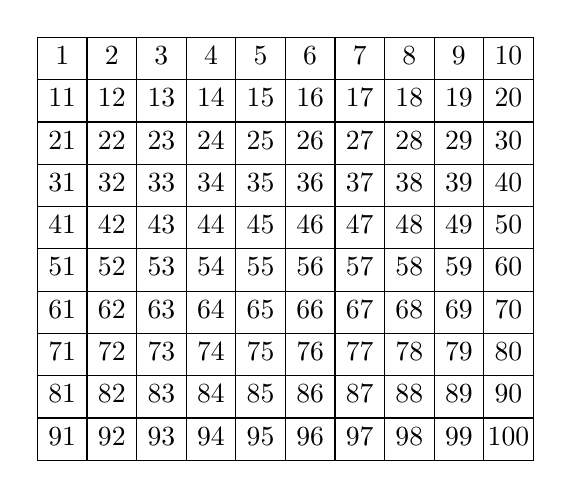
\begin{tikzpicture}

\matrix (first) [table,text width=7mm,name=table]
{
1 & 2 & 3 &4 & 5 & 6 & 7 & 8 & 9 & 10\\
11 & 12 & 13 &14 & 15 & 16 & 17 & 18 & 19 & 20\\
21 & 22 & 23 &24 & 25 & 26 & 27 & 28 & 29 & 30\\
31 & 32 & 33 &34 & 35 & 36 & 37 & 38 & 39 & 40\\
41 & 42 & 43 &44 & 45 & 46 & 47 & 48 & 49 & 50\\
51 & 52 & 53 &54 & 55 & 56 &57 & 58 & 59 & 60\\
61 & 62 & 63 &64 & 65 & 66 & 67 & 68 & 69 & 70\\
71 & 72 & 73 &74 & 75 & 76 & 77 & 78 & 79 & 80\\
81 & 82 & 83 &84 & 85 & 86 & 87 & 88 & 89 & 90\\
91 & 92 & 93 &94 & 95 & 96 & 97 & 98 & 99 & 100\\
};

\end{tikzpicture}
\end{center}

\end{multicols}
\end{esercizio}

\subsubsection*{\thechapter.8 - Criteri di divisibilità}
\begin{esercizio}
\label{ese:1.17}
 Per quali numeri sono divisibili i valori seguenti? Segna i divisori con una crocetta.
\TabPositions{3.5cm}
 \begin{enumeratea}
 \item 1\,320 è divisibile per \tab\fbox{2}\:\fbox{3}\:\fbox{4}\:\fbox{5}\:\fbox{6}\:\fbox{7}\:\fbox{8}\:\fbox{9}\:\fbox{10}\:\fbox{11}
 \item 2\,344 è divisibile per \tab\fbox{2}\:\fbox{3}\:\fbox{4}\:\fbox{5}\:\fbox{6}\:\fbox{7}\:\fbox{8}\:\fbox{9}\:\fbox{10}\:\fbox{11}
 \item 84 è divisibile per \tab\fbox{2}\:\fbox{3}\:\fbox{4}\:\fbox{5}\:\fbox{6}\:\fbox{7}\:\fbox{8}\:\fbox{9}\:\fbox{10}\:\fbox{11}
 \item 1\,255 è divisibile per \tab\fbox{2}\:\fbox{3}\:\fbox{4}\:\fbox{5}\:\fbox{6}\:\fbox{7}\:\fbox{8}\:\fbox{9}\:\fbox{10}\:\fbox{11}
 \item 165 è divisibile per \tab\fbox{2}\:\fbox{3}\:\fbox{4}\:\fbox{5}\:\fbox{6}\:\fbox{7}\:\fbox{8}\:\fbox{9}\:\fbox{10}\:\fbox{11}
 \item 720 è divisibile per \tab\fbox{2}\:\fbox{3}\:\fbox{4}\:\fbox{5}\:\fbox{6}\:\fbox{7}\:\fbox{8}\:\fbox{9}\:\fbox{10}\:\fbox{11}
 \item 792 è divisibile per \tab\fbox{2}\:\fbox{3}\:\fbox{4}\:\fbox{5}\:\fbox{6}\:\fbox{7}\:\fbox{8}\:\fbox{9}\:\fbox{10}\:\fbox{11}
 \item 462 è divisibile per \tab\fbox{2}\:\fbox{3}\:\fbox{4}\:\fbox{5}\:\fbox{6}\:\fbox{7}\:\fbox{8}\:\fbox{9}\:\fbox{10}\:\fbox{11}
 \end{enumeratea}
\end{esercizio}
\pagebreak
\begin{esercizio}
\label{ese:1.18}
 Determina tutti i divisori di 32, 18, 24, 36.
% \begin{multicols}{2}
% \begin{enumeratea}
% \item 32\quad\ldots, \ldots, \ldots, \ldots, \ldots, \ldots, \ldots
% \item 18\quad\ldots, \ldots, \ldots, \ldots, \ldots, \ldots, \ldots
% \item 24\quad\ldots, \ldots, \ldots, \ldots, \ldots, \ldots, \ldots
% \item 36\quad\ldots, \ldots, \ldots, \ldots, \ldots, \ldots, \ldots
% \end{enumeratea}
% \end{multicols}
\end{esercizio}

\subsubsection*{\thechapter.9 - Scomposizione in fattori primi}

\begin{esercizio}[\Ast]
\label{ese:1.19}
Scomponi i seguenti numeri in fattori primi:
 \begin{multicols}{5}
 \begin{enumeratea}
 \item 16;
 \item 18;
 \item 24;
 \item 30;
 \item 32;
 \item 36;
 \item 40;
 \item 42;
 \item 48;
 \item 52;
 \item 60;
 \item 72;
 \item 81;
 \item 105;
 \item 120;
 \item 135;
 \item 180;
 \item 225;
 \item 525;
 \item 360.
 \end{enumeratea}
 \end{multicols}
\end{esercizio}


\begin{esercizio}[\Ast]
\label{ese:1.20}
Scomponi i seguenti numeri in fattori primi:
 \begin{enumeratea}
 \begin{multicols}{5}
 \item 675;
 \item 715;
 \item \np{1900};
 \item \np{1078};
 \item \np{4050};
 \item \np{4536};
 \item \np{12150};
 \item \np{15246};
 \item \np{85050};
 \item \np{138600};
 \item \np{234000};
 \item \np{255000};
 \item \np{293760};
 \item \np{550800};
 \item \np{663552}.
 \end{multicols}
 \end{enumeratea}
\end{esercizio}

\subsubsection*{\thechapter.10 - Massimo Comune Divisore e minimo comune multiplo}

\begin{esercizio}[\Ast]
\label{ese:1.21}
Calcola~$\mcm$ e~$\mcd$ tra i seguenti gruppi di numeri:
\begin{multicols}{3}
 \begin{enumeratea}
 \item 6,~15
 \item 12,~50
 \item 1,~6,~10,~14
 \item 15,~5,~10
 \item 2,~4,~8
 \item 2,~1,~4
 \item 5,~6,~8
 \item 24,~12,~16
 \item 6,~16,~26
 \item 6,~8,~12
 \item 50,~120,~180
 \item 20,~40,~60
 \item 16,~18,~32
 \item 30,~60,~27
 \item 45,~15,~35
 \end{enumeratea}
\end{multicols}
\end{esercizio}

\begin{esercizio}[\Ast]
\label{ese:1.22}
Calcola~$\mcm$ e~$\mcd$ tra i seguenti gruppi di numeri:
\begin{multicols}{3}
 \begin{enumeratea}
 \item 6,~8,~10,~12
 \item 30,~27,~45
 \item 126,~180
 \item 24,~12,~16
 \item 6,~4,~10
 \item 5,~4,~10
 \item 12,~14,~15
 \item 3,~4,~5
 \item 6,~8,~12
 \item 15,~18,~21
 \item 12,~14,~15
 \item 15,~18,~24
 \item 100,~120,~150
 \item 44,~66,~12
 \item 24,~14,~40
 \end{enumeratea}
\end{multicols}
\end{esercizio}

\begin{multicols}{2}
\begin{esercizio}[\Ast]
\label{ese:1.23}
 Tre funivie partono contemporaneamente da una stessa stazione sciistica. La prima compie il tragitto di
andata e ritorno in~15 minuti, la seconda in~18 minuti, la terza in~20. Dopo quanti minuti partiranno di nuovo
insieme?
\end{esercizio}

\begin{esercizio}[\Ast]
\label{ese:1.24}
 Due aerei partono contemporaneamente dall'aeroporto di Milano e vi ritorneranno dopo aver
percorso le loro rotte: il primo ogni~15 giorni e il secondo ogni~18 giorni. Dopo quanti giorni i due
aerei si troveranno di nuovo insieme a Milano?
\end{esercizio}

\begin{esercizio}[\Ast]
\label{ese:1.25}
 Una cometa passa in prossimità della Terra ogni~360 anni, una seconda ogni~240 anni e una terza ogni~750 anni.
 Se quest'anno sono state avvistate tutte e tre, fra quanti anni sarà possibile vederle di nuovo tutte e
tre nello stesso anno?
\end{esercizio}

\begin{esercizio}[\Ast]
\label{ese:1.26}
 Disponendo di~56 penne,~70 matite e~63 gomme, quante confezioni uguali si possono fare? Come sarà
composta ciascuna confezione?
\end{esercizio}
\end{multicols}

\subsubsection*{\thechapter.11 - Espressioni numeriche}

\begin{esercizio}[\Ast]
\label{ese:1.27}
Esegui le seguenti operazioni rispettando l'ordine.
 \begin{multicols}{4}
 \begin{enumeratea}
 \item $15+7-2$;
 \item $16-4+2$;
 \item $18-8-4$;
 \item $16\cdot 2-2$;
 \item $12-2\cdot 2$;
 \item $10-5\cdot 2$;
 \item $20\cdot 4:5$;
 \item $16:4\cdot 2$;
 \item $2+2^2+3$;
 \item $4\cdot 2^3+1$;
 \item $2^4:2-4$;
 \item $(1+2)^3-2^3$;
 \item $\left(3^2\right)^3-3^2$;
 \item $2^4+2^3$;
 \item $2^3\cdot 3^2$;
 \item $3^3:3^2\cdot 3^2$.
 \end{enumeratea}
 \end{multicols}
\end{esercizio}

\subsection{Esercizi riepilogativi}
\begin{esercizio}[\Ast]
Quali delle seguenti scritture rappresentano numeri naturali?
 \begin{multicols}{4}
 \begin{enumeratea}
 \item $5+3-1$;
 \item $6+4-10$;
 \item $5-6+1$;
 \item $7+2-10$;
 \item $2\cdot 5:5$;
 \item $2\cdot 3:4$;
 \item $3\cdot 4-12$;
 \item $12:4-4$;
 \item $11:3+2$;
 \item $27:9:3$;
 \item $18:2-9$;
 \item $10-1:3$.
 \end{enumeratea}
 \end{multicols}
\end{esercizio}


\begin{esercizio}
Calcola il risultato delle seguenti operazioni nei numeri naturali; alcune operazioni non sono
possibili, individuale.
 \begin{multicols}{4}
 \begin{enumeratea}
 \item $5:5=\ldots$;
 \item $5:0=\ldots$;
 \item $1\cdot 5 =\ldots$;
 \item $1-1=\ldots$;
 \item $10:2=\ldots$;
 \item $0:5=\ldots$;
 \item $5\cdot1=\ldots$;
 \item $0:0=\ldots$;
 \item $10:5=\ldots$;
 \item $1:5=\ldots$;
 \item $0\cdot5=\ldots$;
 \item $5:1=\ldots$;
 \item $0\cdot0=\ldots$;
 \item $1\cdot0=\ldots$;
 \item $1:0=\ldots$;
 \item $1:1=\ldots$
 \end{enumeratea}
 \end{multicols}
\end{esercizio}

\begin{esercizio}[\Ast]
Aggiungi le parentesi in modo che l'espressione abbia il risultato indicato.
 \begin{multicols}{2}
 \begin{center}
 ~a)~~$2+5\cdot3+2=35$

 ~b)~~$2+5\cdot3+2=27$
 \end{center}
 \end{multicols}
\end{esercizio}

\begin{esercizio}[\Ast]
Traduci in espressioni aritmetiche le seguenti frasi e calcola il risultato:
 \begin{enumeratea}
 \item aggiungi~12 al prodotto tra~6 e~4;
 \item sottrai il prodotto tra~12 e~2 alla somma tra~15 e~27;
 \item moltiplica la differenza tra~16 e~7 con la somma tra~6 e~8;
 \item al doppio di~15 sottrai la somma dei prodotti di~3 con~6 e di~2 con~5;
 \item sottrai il prodotto di~6 per~4 al quoziente tra~100 e~2;
 \item moltiplica la differenza di~15 con~9 per la somma di~3 e~2;
 \item sottrai al triplo del prodotto di~6 e~2 il doppio del quoziente tra~16 e~4.
 \item il quadrato della somma tra il quoziente intero di~25 e~7 e il cubo di~2;
 \item la somma tra il quadrato del quoziente intero di~25 e~7 e il quadrato del cubo di~2;
 \item la differenza tra il triplo del cubo di~5 e il doppio del quadrato di~5.
 \end{enumeratea}
\end{esercizio}

\begin{esercizio}[\Ast]
 Calcola il valore delle seguenti espressioni:
 \begin{enumeratea}
 \item $(1+2\cdot3):(5-2\cdot2)+1+2\cdot4$;
 \item $ (18-3\cdot2):(16-3\cdot4)\cdot(2:2+2)$;
 \item $2+2\cdot6-[21-(3+4\cdot 3:2)]:2$;
 \item $\lbrace[15-(5\cdot2-4)]\cdot2\rbrace:(30:15+1)-\lbrace[25\cdot4]:10-(11-2)\rbrace$.
 \end{enumeratea}
\end{esercizio}
\pagebreak
\begin{esercizio}[\Ast]
 Calcola il valore delle seguenti espressioni:
 \begin{enumeratea}
 \item $[6\cdot(2\cdot4-2\cdot3)-6]+\lbrace3\cdot(21:7-2)\cdot[(6\cdot5):10]-3\cdot2\rbrace$;
 \item $100:2+3^2-2^2\cdot6$;
 \item $2^7:2^3-2^2$;
 \item $30-5\cdot3+7\cdot2^2-2$.
 \end{enumeratea}
\end{esercizio}

\begin{esercizio}[\Ast]
 Calcola il valore delle seguenti espressioni:
 \begin{enumeratea}
 \item $(3+4)^2-\left(3^2+4^2\right)$;
 \item $5\cdot5^3\cdot5^4:\left(5^2\right)^3+5$;
 \item $32^5:16^4-2^9$;
 \item $\left[3^0+\left(2^4-2^3\right)^2:\left(4^3:4^2\right)+3 \right]:\left(2^6:2^4\right)$.
 \end{enumeratea}
\end{esercizio}


\begin{esercizio}[\Ast]
 Calcola il valore delle seguenti espressioni:
 \begin{enumeratea}
 \item $\left[\left(4^5:4^3\right)-2^3\right]\cdot\left[\left(3^4\cdot 3^3\right):\left(3^2\cdot3\right)\right]:\left(2^2+2^0+3^1\right)$;
 \item $\left(12-5^2:5\right)\cdot4^2:2^3+2^2-1+\left[\left(2^4:2^3\right)^3+4^3:4+2^5\right]:7$;
 \item $\left(5^2\cdot2^2-\left(2^5-2^5:\left(2^2\cdot 3 +4^2:4\right)+2^3\cdot\left(3^2-2^2\right)\right)\right):\left(3\cdot2 \right)\cdot5$;
 \item $\left(3^4\cdot3^3:3^6\right)^2+\left(7^2-5^2\right):2^2~$.
 \end{enumeratea}
\end{esercizio}

\begin{esercizio}[\Ast]
 Calcola il valore delle seguenti espressioni:
 \begin{enumeratea}
 \item $\left(3\cdot2^2-10\right)^4\cdot\left(3^3+2^3\right):7-10\cdot2^3$;
 \item $(195:15)\cdot\left\lbrace \left[3^2\cdot6+3^2\cdot4^2-5\cdot(6-1)^2 \right]\right\rbrace:\left(4^2-3\right)$;
 \item $5+[(16:8)\cdot3+(10:5)\cdot3 ]\cdot\left(2^3\cdot5-1\right)^2-[(3\cdot10):6-1]$;
 \item $\left[4\cdot\left(3\cdot2-3\cdot1^2\right)-5\right]-\left\lbrace 2\cdot(14:7+4):\left[2\cdot(3+2)^2:10+1-4^2:8\right]\right\rbrace~$.
 \end{enumeratea}
\end{esercizio}
\begin{multicols}{2}
 \begin{esercizio}[\Ast]
 Un'automobile percorre~$18\;\unit{km}$ con~1 litro di benzina. Quanta benzina deve aggiungere il proprietario dell'auto
sapendo che l'auto ha già~12~litri di benzina nel serbatoio, che deve intraprendere un viaggio di~$432\;\unit{km}$ e che deve
arrivare a destinazione con almeno~4~litri di benzina nel serbatoio?
\end{esercizio}

\begin{esercizio}[\Ast]
Alla cartoleria presso la scuola una penna costa~3~euro più di una matita. Gianni ha comprato~2~penne e~3~matite e ha speso
16~euro. Quanto spenderà Marco che ha comprato~1~penna e~2~matite?
\end{esercizio}

\begin{esercizio}[\Ast]
 In una città tutte le linee della metropolitana iniziano il loro servizio alla stessa ora. La linea rossa fa una corsa ogni
15~minuti, la linea gialla ogni~20~minuti e la linea blu ogni~30~minuti. Salvo ritardi, ogni quanti minuti le tre linee
partono allo stesso momento?
\end{esercizio}

\begin{esercizio}
 Tre negozi si trovano sotto lo stesso porticato, ciascuno ha un'insegna luminosa intermittente: la prima si spegne ogni
6~secondi, la seconda ogni~5~secondi, la terza ogni~7~secondi. Se le insegne vengono accese contemporaneamente
alle~19:00 e spente contemporaneamente alle~21:00, quante volte durante la serata le tre insegne
si spegneranno contemporaneamente?
\end{esercizio}

\begin{esercizio}
In una gita scolastica ogni insegnante accompagna un gruppo di~12~studenti. Se alla gita partecipano~132~studenti,
quanti insegnanti occorrono?
\end{esercizio}

\begin{esercizio}
Un palazzo è costituito da~4~piani con~2~appartamenti per ogni piano. Se ogni appartamento ha~6~finestre con~4~vetri
ciascuna, quanti vetri ha il palazzo?
\end{esercizio}

\begin{esercizio}
Spiega brevemente il significato delle seguenti parole:

a)~numero~primo,\quad b)~numero~dispari,

c)~multiplo,\quad d)~cifra.
% \begin{enumeratea}
% \item numero primo;
% \item numero dispari;
% \item multiplo;
% \item cifra.
% \end{enumeratea}
\end{esercizio}

\begin{esercizio}
Rispondi brevemente alle seguenti domande:
 \begin{enumeratea}
 \item cosa vuol dire scomporre in fattori un numero?
 \item ci può essere più di una scomposizione in fattori di un numero?
 \item cosa vuol dire scomporre in fattori primi un numero?
 \item che differenza c'è tra la frase ``$a$ e $b$ sono due numeri primi'' e la frase ``$a$ e $b$ sono primi tra di loro''?
 \end{enumeratea}
\end{esercizio}
\end{multicols}

\subsection{Risposte}

\paragraph{\thechapter.11.}
a)~$6^6$,\quad b)~$5^4$,\quad c)~1,\quad d)~$6^3$.

\paragraph{\thechapter.19.}
a)~$2^4$,\quad b)~$ 2\cdot 3^2 $,\quad c)~$ 2^3 \cdot 3 $,\quad d)~$ 2\cdot 3\cdot 5 $,\quad e)~$ 2^5 $,\quad f)~$ 2^2 \cdot 3^2 $,\quad g)~$ 2^3 \cdot 5 $,\quad h)~$ 2\cdot 3\cdot 7 $,\quad i)~$ 2^4 \cdot 3 $,\quad j)~$ 2^2 \cdot 13 $,\quad k)~$ 2^2 \cdot 3 \cdot5 $,\quad l)~$ 2^3 \cdot 3^2 $,\quad m)~$ 3^4 $,\quad n)~$ 3\cdot 5\cdot 7 $,\quad o)~$ 2^3 \cdot 3\cdot 5 $,\quad p)~$ 3^3 \cdot 5 $,\quad q)~$ 2^2 \cdot 3^2 \cdot 5 $,\quad r)~$ 2^2 \cdot 5^2 $, s)~$3\cdot5^2\cdot7$,\quad t)~$ 2^3 \cdot 3^2 \cdot5$.

\paragraph{\thechapter.20.}
d)~$2\cdot7^2\cdot11$,\quad e)~$2\cdot3^4\cdot5^2$,\quad f)~$2^3\cdot3^4\cdot7$,\quad g)~$2\cdot3^5\cdot5^2$,\quad h)~$2\cdot3^2\cdot7\cdot11^2$,\quad i)~$2\cdot3^5\cdot5^2\cdot7$,\quad
j)~$2^3\cdot3^2\cdot5^2\cdot7\cdot11$,\quad k)~$2^4\cdot3^2\cdot5^3\cdot13$,\quad l)~$2^3\cdot3\cdot5^4\cdot17$,\quad m)~$2^7\cdot3^3\cdot5\cdot17$,\quad n)~$2^4\cdot3^4\cdot5^2\cdot17$,\quad o)~$2^{13}\cdot3^4$.

\paragraph{\thechapter.21.}
a)~30;~3,\quad b)~300;~2,\quad c)~210;~1,\quad d)~30;~5,\quad e)~8;~2,\quad f)~4;~1,\quad g)~120;~1,\quad k)~1800;~10,\quad l)~120;~20.

\paragraph{\thechapter.22.}
m)~600;~10,\quad n)~132;~2,\quad o)~840;~2.

\begin{multicols}{3}
\paragraph{\thechapter.23.}
3 ore.

\paragraph{\thechapter.24.}
90 giorni.

\paragraph{\thechapter.25.}
$ \np{18000}$~anni.
\end{multicols}

\paragraph{\thechapter.26.}
7 confezioni, ognuna conterrà 8~penne, 10~matite, e 9~gomme.

\paragraph{\thechapter.27.}
a)~20,\quad e)~8,\quad i)~9,\quad m)~720.

\paragraph{\thechapter.28.}
a, b, e, g, j, k.

\paragraph{\thechapter.30.}
a)~$ (2+5)\cdot(3+2) $,\quad b)~$ 2+5\cdot(3+2) $.

\paragraph{\thechapter.31.}
a)~36,\quad b)~18,\quad c)~126,\quad d)~2,\quad e)~26,\quad f)~30.

\begin{multicols}{2}
\paragraph{\thechapter.32.}
a)~16,\quad b)~9,\quad c)~8,\quad d)~5.

\paragraph{\thechapter.33.}
a)~9,\quad b)~35,\quad c)~12,\quad d)~41.

\paragraph{\thechapter.34.}
a)~24,\quad b)~30,\quad c)~0,\quad d)~5.

\paragraph{\thechapter.35.}
a)~81,\quad b)~25,\quad c)~25,\quad d)~15.

\paragraph{\thechapter.36.}
a)~0,\quad b)~73,\quad c)~$18\,253$,\quad d)~4.

\paragraph{\thechapter.37.}
Almeno~16.

\paragraph{\thechapter.38.}~9~euro.

\paragraph{\thechapter.39.}~60~minuti.
\end{multicols}
% EOF


\cleardoublepage
